\documentclass[12pt,a4paper,twoside]{report}

%%%%%%%%%%%%%%%%%%%%%%%%%%%%%%%%%%%%%%%%%%%%%%%%%%%%%%%%%%%%%%%%%%%%%%%%%%%%%

% Definitions for the title page

\newcommand{\reporttitle}{Lip Reading in 3D}
\newcommand{\reportauthor}{Peter Robertson}
\newcommand{\supervisor}{Dr Stefanos Zafeiriou}
\newcommand{\degreetype}{Computing Science / Machine Learning}

%%%%%%%%%%%%%%%%%%%%%%%%%%%%%%%%%%%%%%%%%%%%%%%%%%%%%%%%%%%%%%%%%%%%%%%%%%%%%

% load some definitions and default packages
%%%%%%%%%%%%%%%%%%%%%%%%%%%%%%%%%%%%%%%%%
% University Assignment Title Page 
% LaTeX Template
% Version 1.0 (27/12/12)
%
% This template has been downloaded from:
%%%%%%%%%%%%%%%%%%%%%%%%%%%%%%%%%%%%%%%%%
%----------------------------------------------------------------------------------------
%	PACKAGES AND OTHER DOCUMENT CONFIGURATIONS
%----------------------------------------------------------------------------------------

\usepackage[nottoc,notlot,notlof]{tocbibind}
\usepackage[T1]{fontenc}
%\usepackage{hyperref}
\usepackage{indentfirst}
\usepackage{amsmath}
\usepackage{amssymb}
\usepackage{graphicx}
\usepackage{subcaption}
\usepackage{geometry}
 \geometry
 {
     a4paper,
     left=25mm,
     right=25mm,
     top=30mm,
     bottom=30mm,
 }

% \usepackage[a4paper,hmargin=2.8cm,vmargin=2.0cm,includeheadfoot]{geometry}
\usepackage{textpos}
\usepackage{natbib} % for bibliography
%\usepackage{tabularx,longtable,multirow,subfigure,caption}
\usepackage{fncylab} %formatting of labels
\usepackage{fancyhdr} % page layout
\usepackage{url} % URLs
\usepackage[english]{babel}
%\usepackage{dsfont}
\usepackage{epstopdf}
\usepackage{backref} % needed for citations
\usepackage{array}
\usepackage{latexsym}
\usepackage[pdftex,pagebackref,hypertexnames=false,colorlinks]{hyperref} % provide links in pdf
 
\hypersetup{pdftitle={},
  pdfsubject={}, 
  pdfauthor={},
  pdfkeywords={}, 
  pdfstartview=FitH,
  pdfpagemode={UseOutlines},% None, FullScreen, UseOutlines
  bookmarksnumbered=true, bookmarksopen=true, colorlinks,
    citecolor=black,%
    filecolor=black,%
    linkcolor=black,%
    urlcolor=black}
 
\usepackage[all]{hypcap}
\frenchspacing

\DeclareMathOperator{\tr}{tr}

% load some macros
% Here, you can define your own macros. Some examples are given below.

\newcommand{\R}[0]{\mathds{R}} % real numbers
\newcommand{\Z}[0]{\mathds{Z}} % integers
\newcommand{\N}[0]{\mathds{N}} % natural numbers
\newcommand{\C}[0]{\mathds{C}} % complex numbers
\newcommand{\bm}[1]{{\boldsymbol{{#1}}}} % vector
\newcommand{\mat}[1]{{\boldsymbol{{#1}}}} % matrix

\newcommand{\E}[1]{\mathbb{E}_{#1}} % Expectation
\newcommand{\Pd}[1]{\mathbb{P}_{#1}} % Probability Distribution


\date{September 2019}

\begin{document}

% load title page
\begin{titlepage}

\newcommand{\HRule}{\rule{\linewidth}{0.5mm}} % Defines a new command for the horizontal lines, change thickness here


%----------------------------------------------------------------------------------------
%	LOGO SECTION
%----------------------------------------------------------------------------------------

%
\includegraphics[width = 4cm]{../figures/imperial} \\ [0.5] 
\center

%----------------------------------------------------------------------------------------
%	HEADING SECTIONS
%----------------------------------------------------------------------------------------

\textsc{\Large Imperial College London}\\[0.5cm] 
\textsc{\large Department of Computing}\\[0.5cm] 

%----------------------------------------------------------------------------------------
%	TITLE SECTION
%----------------------------------------------------------------------------------------

\HRule \\[0.4cm]
{ \huge \bfseries \reporttitle}\\ % Title of your document
%{ \huge \bfseries Report Title}\\ % Title of your document
\HRule \\[1.5cm]
 
%----------------------------------------------------------------------------------------
%	AUTHOR SECTION
%----------------------------------------------------------------------------------------

\begin{minipage}{0.4\textwidth}
\begin{flushleft} \large
\emph{Author:}\\
\reportauthor % Your name
\end{flushleft}
\end{minipage}
~
\begin{minipage}{0.4\textwidth}
\begin{flushright} \large
\emph{Supervisor:} \\
\supervisor % Supervisor's Name
\end{flushright}
\end{minipage}\\[4cm]


%----------------------------------------------------------------------------------------
%	FOOTER & DATE SECTION
%----------------------------------------------------------------------------------------
\vfill % Fill the rest of the page with whites pace
Submitted in partial fulfilment of the requirements for the MSc degree in \degreetype~of Imperial College London\\[0.5cm]
%degree \\[0.5cm]

\makeatletter
%\@date 
\makeatother


\end{titlepage}



% page numbering etc.
\pagenumbering{roman}
\clearpage{\pagestyle{empty}\cleardoublepage}
\setcounter{page}{1}
\pagestyle{fancy}

\fancyhf{}
\fancyfoot[C]{\thepage}
\fancyhead[RE]{\nouppercase{\leftmark}}
\fancyhead[LO]{\nouppercase{\rightmark}}

%%%%%%%%%%%%%%%%%%%%%%%%%%%%%%%%%%%%
\begin{abstract}
Lip reading is a skill which is renowned for being challenging for humans, with few individuals being capable of implementing the skill successfully.
Recent successes have been made in training Machine Learning models to predict speech from video inputs which have been able to outperform human level accuracy.
Currently however, no models exist which have attempted to use 3D data of facial scans for the use of lip reading.
In this report lip reading is successfully implemented with the use of 3D facial scans to make predictions on a word level with above 50\% mean test accuracy on 500 labels, forming the baseline for future work to build upon.
The current lack of datasets suitable for this research is the dominant problem in this field of research.
In addition to the task of lip reading from 3D facial scans, solving this secondary problem is also attempted.
To resolve this issue, the use of Generative Adversarial Networks is investigated as a means of generating 3D facial data corresponding to an audio input.
\end{abstract}

\cleardoublepage
%%%%%%%%%%%%%%%%%%%%%%%%%%%%%%%%%%%%
\section*{Acknowledgements}
I would like to thank the support of my supervisor; Dr Stefanos Zafeiriou, for his words of advice and guidance in this project.

Secondly I would like to thank the researchers for assisting with support, resources and advice; Athanasios Papaioannou, Evangelos Ververas and Panagiotis Tzirakis.

\clearpage{\pagestyle{empty}\cleardoublepage}

%%%%%%%%%%%%%%%%%%%%%%%%%%%%%%%%%%%%
%--- table of contents
\tableofcontents 
\listoffigures
\listoftables


\clearpage{\pagestyle{empty}\cleardoublepage}
\pagenumbering{arabic}
\setcounter{page}{1}

%%%%%%%%%%%%%%%%%%%%%%%%%%%%%%%%%%%%
%\linenumbers
\chapter{Introduction}

Whole section needs rewriting...

Visual speech prediction, often referred to as lip reading, is a very difficult task, partly due to ambiguities between phonemes such as '\textit{p}' and '\textit{b}', which look the same but sound different.
Current methods of addressing this problem focus on training deep learning models using 2D temporal data of people speaking with the relevant video frames labelled with the correct spoken text \cite{Chung2016, Assael2016, Chung2017, Shillingford2018}.
There currently do not exist any models which attempt to address this problem with the use of 3D temporal datasets made up of head scans of subjects, capturing depth and thus, more information of the mouth which may be of use to the models.
However, there currently exists a severe lack of availability of such datasets due to the complexity and hardware requirements in capturing such data.
Currently their exists two publicly available datasets: LRW-3D \cite{Tzirakis2019} and the VOCASET \cite{Cudeiro2019}, both of which are relatively small in comparison to the models used in current lip reading models.
To first attempt this problem, new datasets which capture 3D temporal models of subjects heads speaking must be established by the community.
As well as capturing new data, expanding existing datasets with generated synthetic data with the use of generative adversarial networks may assist in the solution to this problem.

In an attempt to add variation to sampled generated from a model, a Generative Adversarial Network is proposed which can be trained end-to-end from audio inputs to drive a 3D template mesh.
This shall be achieved by initially using the...

\begin{itemize}

    \item What is the problem?
    \item Current solutions
    \item Issues with current solutions
    \item Your observation / proposition

\end{itemize}

%%%%%%%%%%%%%%%%%%%%%%%%%%%%%%%%%%%%
\chapter{3D Facial Modelling Background}

This chapter shall discuss the preliminary background theory on 3D Facial Modelling and how this data is processed and represented for use with Deep Learning models.
As the data captured by 3D facial scans is made of a high dimensional point cloud, each point having an position in the $x, y$ and $z$ dimension, a lower dimensional representation of the data can be found which retains the variance in the data.
This can be achieved with the use of Blendshape Axis, found with Principal Component Analysis (PCA).
In order to remove unwanted variance in the data from facial movement not correlated with speech, such as head movement, the data samples should first be brought into correspondence (also known as alignment or registration) to remove these undesirable variations in the data.
This is achieved with the use of Procrustes Analysis.

\section{Data Collection and Representation}
Unlike 2D video where the subject is captured from a single angle without any depth information, 3D models cannot be captured with a single camera.
In most instances, 3D head scans are captured with the use of a multi-camera rig with multiple cameras capturing video simultaneously.
The number and type of cameras can vary from system to system, but the principle remains consistent.
All cameras must be synchronised to capture footage at the same time, with the same frame rate.
This is inherently a more complex system than 2D video capture as is therefore more expensive, limiting the accessibility of such systems.  
Once the images have been captured, the footage must be combined in order to produce a 3D model of the subject's head \cite{Li2017}, often referred to as a facial mesh.
A facial mesh is made up of a point cloud of vertices and vertex connections.
Depending on the resolution of the system used to capture the data, the number of points which are used to represent the subject can vary, each with $x$, $y$ and $z$ coordinates in space.
Depending on the mesh capture pipeline, the number of vertices may vary, but even a low resolution mesh may contain several thousand vertices.
In the example shown in Figure \ref{fig:FLAME_Point_Cloud}, the FLAME model \cite{Li2017} uses around 5000 vertex positions, each with an $(x, y, z)$ value, resulting in a total of 15,000 parameters for a single capture in time.
While Deep Learning models have been trained to drive all vertex positions from a starting template mesh \cite{Karras2017a}, a simpler representation can be achieved with the use of Blendshapes.

\begin{figure}[h]
    \centering
    \begin{subfigure}[b]{0.22\textwidth}
        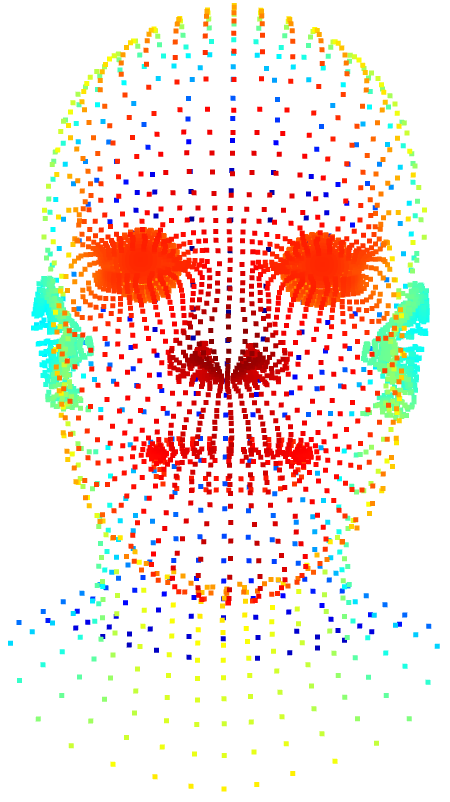
\includegraphics[width=\textwidth]{figures/dataset/flame_front.png}
    \end{subfigure}
    \hfill
    \begin{subfigure}[b]{0.31\textwidth}
        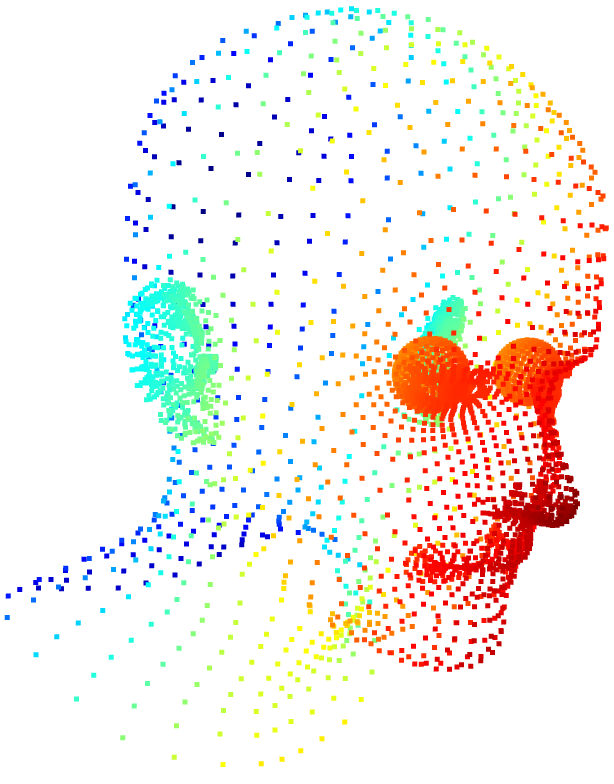
\includegraphics[width=\textwidth]{figures/dataset/flame_angle.png}
    \end{subfigure}
    \hfill
    \begin{subfigure}[b]{0.28\textwidth}
        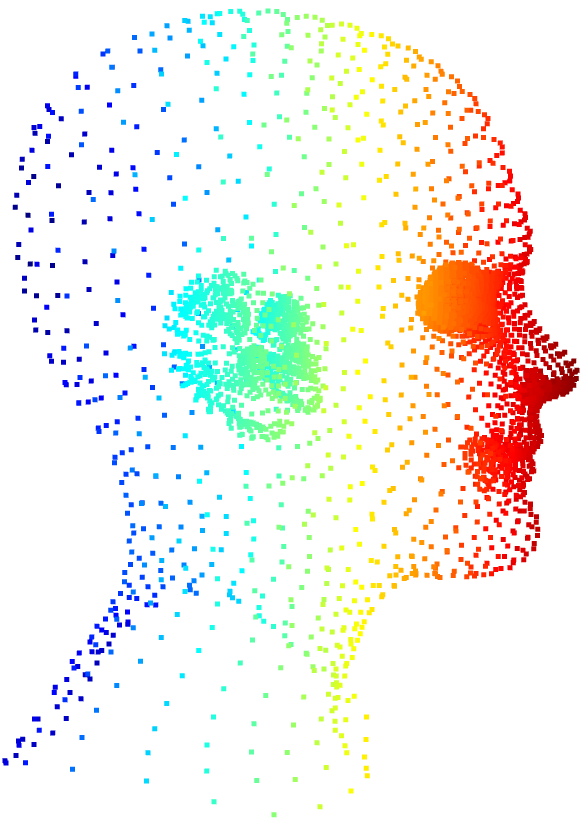
\includegraphics[width=\textwidth]{figures/dataset/flame_side.png}
    \end{subfigure}
    \caption{Point Cloud Representation of FLAME Model \cite{Li2017}}\label{fig:FLAME_Point_Cloud}
\end{figure}

\subsection{Blendshapes} \label{blendshapes}
Capturing realistic facial motion by modelling the displacements of all of these vertices is impractical when manipulating a model by hand and may hinder the performance of a Machine Learning model due to the high dimensionality of the data.
Blendshapes attempt to model aspects of realistic facial motion by finding the relations between these vertices and manipulating them simultaneously \cite{Lewis2010}; by reducing the number of parameters, the model becomes more manageable to control.
One method of producing model Blendshapes is with the use of PCA.
By applying PCA on a dataset of facial meshes, the resulting principle components represent the changes in facial motion which capture the largest amount of variation in the set whilst reducing the number of model parameters substantially.

\subsubsection{Principal Component Analysis} \label{sec:pca}
Given a collection of measured data points in a high dimensional space, it is often desirable to reduce the dimensionality of such data to a lower dimensional latent space, in order to aid processing the data or enable visualisation.
In such instances, it is desirable for the mapping to the latent space to maintain as much information from the original data as possible.

PCA aims to reduce the dimensionality of a collection of data points while maximising the variance in the latent space.
Alternatively, PCA aims to find a mapping from the original data to a new latent space which allow for the original data to be reconstructed with minimal error.
These two aims are in fact equivalent.

Let $\bm{x_i} \in \mathbb{R}^f$ represent a data point in $f$ dimensional space and $\bm{y_i} \in \mathbb{R}^d$ represent the point which $\bm{x_i}$ is transformed to by a linear transformation $\mat{W}$ equation (\ref{eq:pca_transformation}), where $d << f$.

\begin{equation} \label{eq:pca_transformation}
    \bm{y_i} = \mat{W}^\top \bm{x_i}
\end{equation}
where,

\begin{equation*}
    \bm{y_i} = \begin{bmatrix} 
                y_{i1} \\
                \vdots \\
                y_{id} 
               \end{bmatrix},
    \quad
    \bm{x_i} = \begin{bmatrix} 
                \bm{x}_{i1} \\
                \vdots \\
                \bm{x}_{if} 
               \end{bmatrix},
    \quad
    \mat{W} = [
               \bm{w_1}, \dots, \bm{w_d}
              ],
    \quad
    \bm{w_i} = \begin{bmatrix} 
                w_{i1} \\
                \vdots \\
                w_{if} 
               \end{bmatrix}
\end{equation*}

\bigskip
The optimal transformation $\mat{W}$ will maximise the variance in the data, where variance is expressed by equation (\ref{eq:variance}).
This then follows that the optimal solution is found by maximising equation (\ref{eq:pca_optimum_transformation}).
To prevent the trivial solution where $\bm{w}_k = \infty$, constrain a fixed magnitude $\mat{W}^\top \mat{W} = \mat{I}$.


\begin{equation} \label{eq:variance}
    \sigma_y^2 = \frac{1}{N} \sum_{i=1}^{N} (y_{ik} - \mu_k)^2
\end{equation}
where,
\begin{equation*}
    \mu_k = \frac{1}{N} \sum_{i=1}^N y_{ik}
\end{equation*}

\begin{align*}
    \mat{W} &=\operatorname*{arg}\operatorname*{max}_\mat{W} 
                \frac{1}{N} \sum_{k=1}^{d} \sum_{i=1}^{N} 
                (y_{ik} - \mu_k)^2 \\
            &=\operatorname*{arg}\operatorname*{max}_\mat{W} 
                \frac{1}{N} \sum_{k=1}^{d} \sum_{i=1}^{N} 
                \bm{w}_k^\top 
                (\bm{x}_i - \bm{\mu})
                (\bm{x}_i - \bm{\mu})^\top 
                \bm{w}_k \\
            &=\operatorname*{arg}\operatorname*{max}_\mat{W} 
                \sum_{k=1}^{d}
                \bm{w}_k^\top 
                \mat{S}_t
                \bm{w}_k \\
\end{align*}
where $\mat{S}_t$ is the covariance matrix,
\begin{equation} \label{eq:covariance}
    \mat{S}_t = \frac{1}{N} \sum_{i=1}^{N} 
                (\bm{x}_i - \bm{\mu})
                (\bm{x}_i - \bm{\mu})^\top 
\end{equation}
and,
\begin{equation*}
    \bm{\mu} = \frac{1}{N} \sum_{i=1}^N \bm{x}_i
\end{equation*}


\begin{equation} \label{eq:pca_optimum_transformation}
    \mat{W} = \operatorname*{arg}\operatorname*{max}_\mat{W} 
          \tr[\mat{W}^\top \mat{S}_t \mat{W}],
          \quad
    \text{subject to} \quad 
    \mat{W}^\top \mat{W} = \mat{I}
\end{equation}

\bigskip
By constructing the Lagrangian from equation (\ref{eq:pca_optimum_transformation}) and solving, the solution in equation (\ref{eq:pca_solved}) can be obtained.
From eigendecomposition, $\mat{W}$ has columns of eigenvectors which correspond to the $d$ largest non-zero eigenvalues of the covariance matrix, $\mat{S}_t$.

\begin{equation*}
    L(\mat{W}, \mat{\Lambda}) = \tr[\mat{W}^\top \mat{S}_t \mat{W}] - \tr[\Lambda(\mat{W}^\top \mat{W} - \mat{I})]
\end{equation*}

\begin{equation*}
    \frac{\partial \tr[\mat{W}^\top \mat{S}_t \mat{W}]}{\partial \mat{W}} = 2 \mat{S}_t \mat{W},
    \quad
    \frac{\partial \tr[\Lambda(\mat{W}^\top \mat{W} - \mat{I})]}{\partial \mat{W}} = 2 \mat{W \Lambda}
\end{equation*}

\begin{equation*}
    L(\mat{W}, \mat{\Lambda}) = 0 
\end{equation*}

\begin{equation} \label{eq:pca_solved}
    \mat{S}_t \mat{W} = \mat{W \Lambda}
\end{equation}

\section{Facial Mesh Alignment}
In order to create Blendshapes from 3D facial scans, movement within scans should be limited to facial movement with as little head movement as possible.
If head movement remains within the scans, then this will be reflected in the principal axis produced by PCA and as head motion is independent from speech, this is undesirable.
Initial data capture can aim to minimise subject head movement, however this cannot be completely eliminated.
To remove head motion from the dataset, the scans can be brought into alignment relative to landmark positions on the face which do not move during speech.
Such landmarks include the nose, corners of the eyes and cheek bones, as these points will be stationary during speech.
By aligning the meshes based on the variation in these points, the head position of the subjects can be constrained while the mouths are not.
To achieve this, Procrustes Analysis can be used.

\subsection{Procrustes Analysis} \label{sec:procrustes_analysis}
Procrustes Analysis is a statistical shape analysis method used to analyse the differences between two objects \cite{Krzanowski2000}.
Given matrices $\mat{X} \in \mathbb{R}^{(n\times f)}$ and $\mat{Y} \in \mathbb{R}^{(n\times f)}$, each representing the coordinates of $n$ points in an $f$-dimensional feature space, a common statistical difference metric is the sum of square differences (\ref{eq:ssd}).
\begin{equation}
    \label{eq:ssd}
    D = \sum_{i=1}^{n} \sum_{j=1}^{f} (x_{ij} - y_{ij})^2
\end{equation}

However, two objects which are mathematically similar can still have a significant difference when they are scaled differently and are in different positions and orientations in space.
In order to compare two objects regardless of these factors, the differences in orientation, scale and spacial position of the objects must be minimised by bringing the objects into optimal alignment.

\subsubsection{Translational Alignment} \label{sec:trans_align}
Translational components can be eliminated by having the centroids of the two objects lie at the same position in space.
This can be easily achieved by subtracting the mean of each object's points from itself such that the centroid now lies at the origin.

Let $\bar{x}_j = \frac{1}{n} \sum_{i=1}^{n} x_{ij}$ and $\bar{y}_j = \frac{1}{n} \sum_{i=1}^{n} y_{ij}$, where $(j = 1, \dots, f)$ represent the mean of each feature, such that the centroids of the two objects are given by $C_X = (\bar{x}_1, \bar{x}_2, \dots, \bar{x}_f)$ and $C_Y = (\bar{y}_1, \bar{y}_2, \dots, \bar{y}_f)$ respectively.
By subtracting the mean of $\mat{X}$ and $\mat{Y}$ from themselves, the centroids $C_X$ and $C_Y$ will be in alignment at the origin, minimising the sum of square differences due to translational components.

\subsubsection{Scaling Alignment} \label{sec:scale_align}
Similarly, scaling components can be removed by rescaling the objects by the root mean square distance (\ref{eq:rms}), such that the root mean square distance will be of unit distance for both.

\begin{equation}
    \label{eq:rms}
    D = \sqrt{\frac{1}{n} \sum_{i=1}^{n} \sum_{j=1}^{f} x_{ij}^2}
\end{equation}

\subsubsection{Rotational Alignment} \label{sec:rot_align}
In order to align the objects to the same orientation, a rotational matrix which is able to map $\mat{X}$ to $\mat{Y}$ as closely as possible must be found.
This is described as the Orthogonal Procrustes problem and can be solved with Singular Value Decomposition (SVD).
Given matrices $\mat{A}$ and $\mat{B}$, the orthogonal matrix $\mat{R}$ is the matrix which matches $\mat{A}$ to $\mat{B}$ as closely as possible, as described by equation (\ref{eq:orth_proc_prob}), where $\| \cdot \|_F$ is the Fobius norm.

\begin{equation}
    \label{eq:orth_proc_prob}
    \mat{R} =\operatorname*{arg}\operatorname*{min}_\mat{\Omega} 
        \| \mat{\Omega} \mat{A} - \mat{B} \|_F
        \quad
        \text{subject to}
        \quad
        \mat{\Omega}^\top \mat{\Omega} = \mat{I}
\end{equation}

The product of matrices $\mat{A}$ and $\mat{B}$ can be decomposed (\ref{eq:svd_2}), and then the rotational matrix $\mat{R}$ can be expressed (\ref{eq:proc_rotation}).
\begin{equation} \label{eq:svd_1}
    \mat{M} = \mat{B} \mat{A}^\top
\end{equation}
\begin{equation} \label{eq:svd_2}
    \mat{M} = \mat{U} \mat{\Sigma} \mat{V}^\top
\end{equation}
\begin{equation} \label{eq:proc_rotation}
    \mat{R} = \mat{U} \mat{V}^\top
\end{equation}

\subsubsection{A Simple Application of Procrustes Analysis}
This section follows the steps of object alignment using Procrustes Analysis as described above with a simple example.
A pair of configurations are given by the matrices below, visualised in Figure \ref{fig:procrustes_ex_1}.

\begin{equation*}
    \mat{X} = 
    \begin{pmatrix} 
        1 & 1 \\
        1 & 2 \\
        3 & 2
    \end{pmatrix}
    \quad 
    \text{and} 
    \quad 
    \mat{Y}
    \begin{pmatrix} 
        -3 & -2 \\
        -3 & -4 \\
        -7 & -4
    \end{pmatrix}
\end{equation*}

\begin{figure*}[h]
    \centering
    \begin{subfigure}[b]{0.475\textwidth}
        \centering
        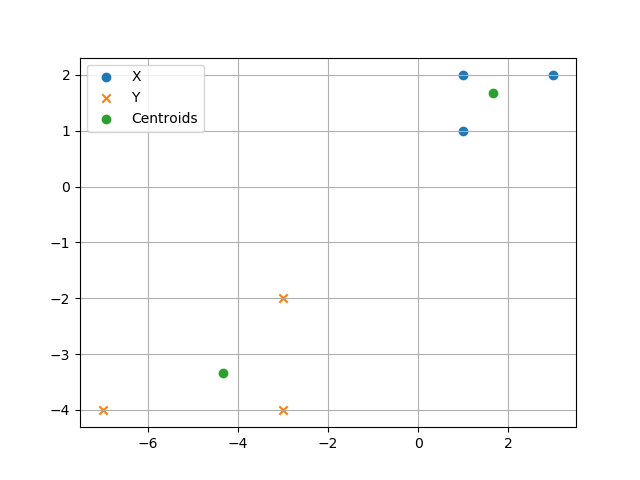
\includegraphics[width=\textwidth]{figures/procrustes/procrustes_ex1}
        \caption[]
        {{\small Original coordinates}}    
        \label{fig:procrustes_ex_1}
    \end{subfigure}
    \begin{subfigure}[b]{0.475\textwidth}  
        \centering 
        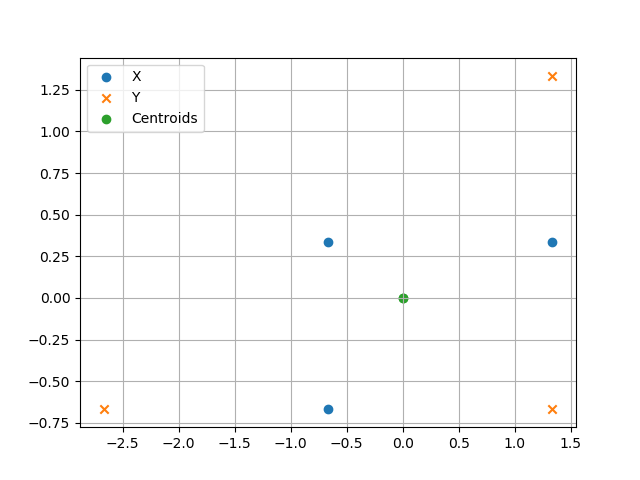
\includegraphics[width=\textwidth]{figures/procrustes/procrustes_ex2}
        \caption[]
        {{\small Translation}}    
        \label{fig:procrustes_ex_2}
    \end{subfigure}
    \begin{subfigure}[b]{0.475\textwidth}   
        \centering 
        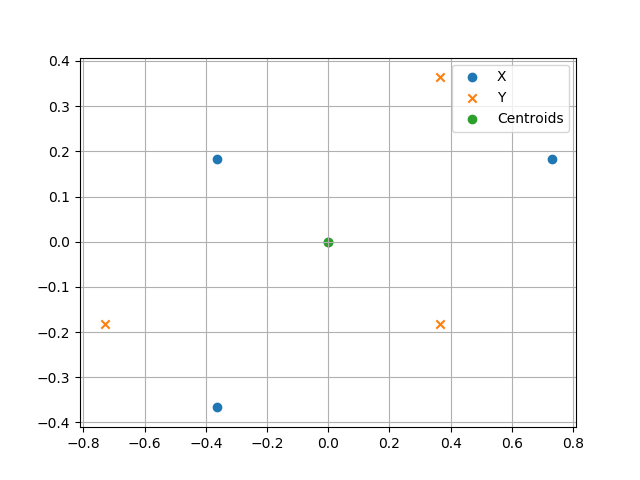
\includegraphics[width=\textwidth]{figures/procrustes/procrustes_ex3}
        \caption[]
        {{\small Scaling}}    
        \label{fig:procrustes_ex_3}
    \end{subfigure}
    \begin{subfigure}[b]{0.475\textwidth}   
        \centering 
        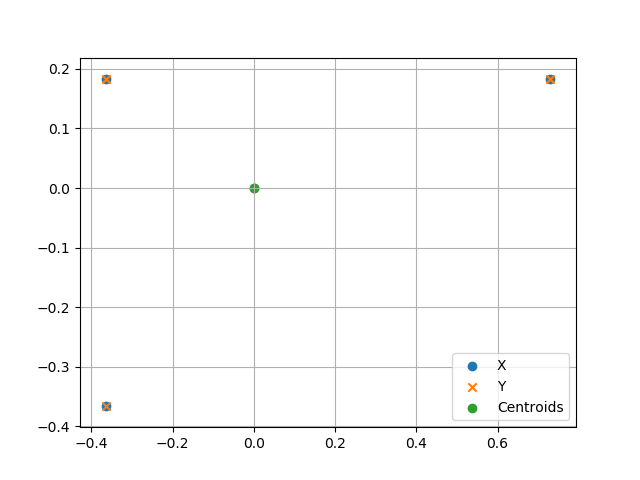
\includegraphics[width=\textwidth]{figures/procrustes/procrustes_ex4}
        \caption[]
        {{\small Rotation}}    
        \label{fig:procrustes_ex_4}
    \end{subfigure}
    \caption[]
    {Application of Procrustes Analysis} 
    \label{fig:procrustes_analysis}
\end{figure*}

Before applying alignment, the sum of square differences between $\mat{X}$ and $\mat{Y}$ is
\begin{align*}
    D& = {(1+3)^2 + (1+2)^2} + {(1+3)^2 + (2+4)^2} + {(3+7)^2 + (2+4)^2} \\
     & = 213
\end{align*}
As described in section (\ref{sec:trans_align}), the initial objects are translated so that their centroids lie at the origin (Figure \ref{fig:procrustes_ex_2}). This is then followed by scaling alignment and finally rotational alignment (Figures \ref{fig:procrustes_ex_3}, \ref{fig:procrustes_ex_4}).
After alignment, the difference is zero as these objects are both similar triangles.

\subsection{Procrustes Analysis for Facial Mesh Alignment}
The process of Procrustes Analysis described above deals with objects in which all coordinate points are used to find the optimum alignment, however this is inappropriate for facial mesh alignment as not only would the position of the head be aligned to, but so would the motion from speech, of which the aim is to maintain variation.
However, a subset of points of a pair of objects can be used to align the entire object.
By selecting points which do not contain any movement due to speech or facial expression, variation in these points can be assumed to be only from head motion.
Such positions include the nose, corners of the eyes and cheekbones.
If the facial scans captures 360 degrees, then points on the back of the subject's head can also be used.
From this subset of points, the translation, scaling and rotational matrix can be found which aligns these points using the steps described in section \ref{sec:procrustes_analysis} but then applied to the entire object.
An example of such an application is shown in Figure \ref{fig:VOCASET_Alignment} before and after alignment has been applied.

\begin{figure}[h]
    \centering
    \begin{subfigure}[b]{0.4\textwidth}
        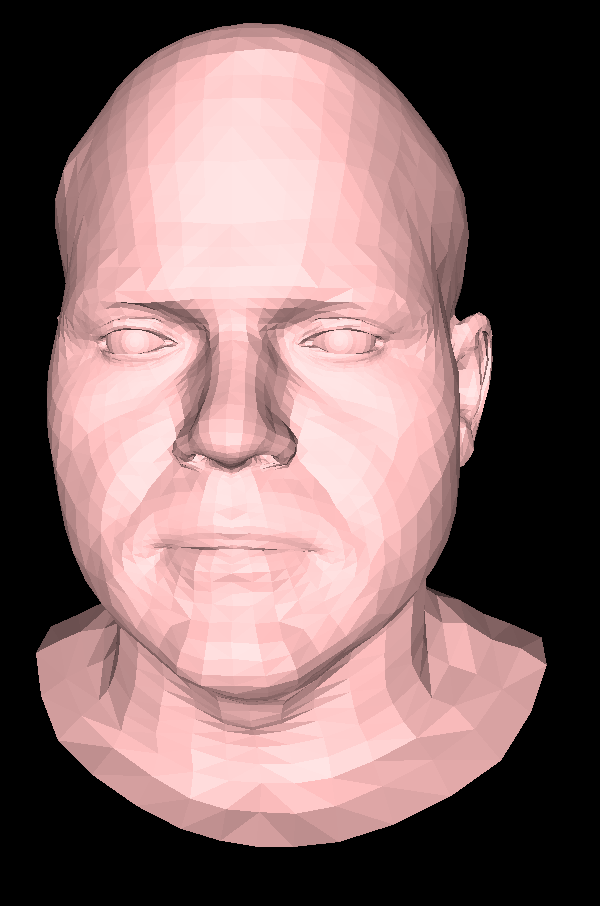
\includegraphics[width=\textwidth]{figures/dataset/subject2_unaligned.png}
        \caption{Before Alignment}
    \end{subfigure}
    \begin{subfigure}[b]{0.4\textwidth}
        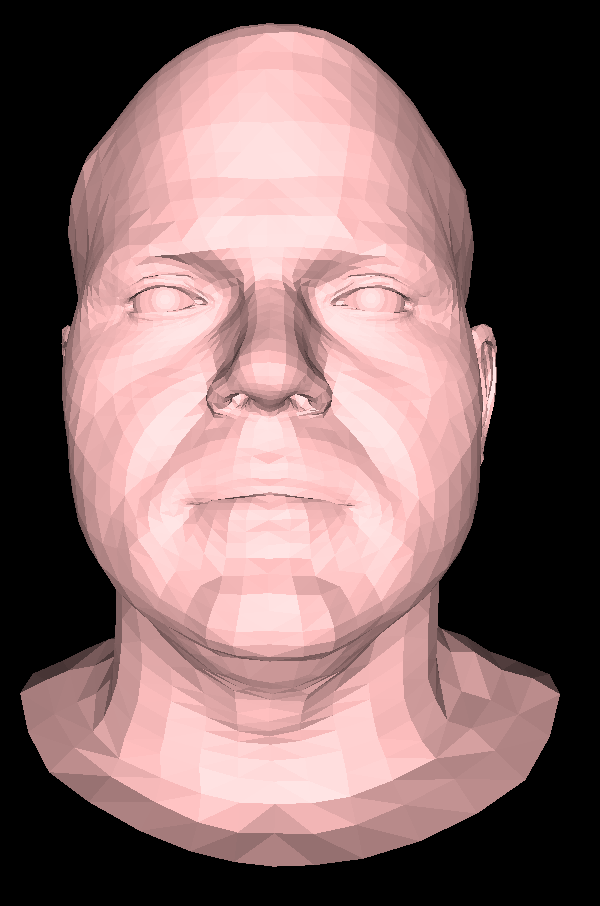
\includegraphics[width=\textwidth]{figures/dataset/subject2_aligned.png}
        \caption{After Alignment}
    \end{subfigure}
    \caption{Procrustes Alignment Applied to VOCASET \cite{Cudeiro2019}}\label{fig:VOCASET_Alignment}
\end{figure}

\section{Chapter Summary}
This chapter has provided an overview of the process of PCA and how the calculated principal axis from this analysis can be used as Blendshape Axis, along which a facial model can be interpolated to describe variation in the dataset.
Secondly, an overview of the background mathematics used to align a dataset made up of 3D facial scans can be brought into correspondence such that all data samples are scaled to the same size at the same position and are aligned to a collection of points which should remain fixed throughout the data.
This allows for remaining variation in the data to be present in only the desired attributes, such as movement in subjects mouth while removing variation in head movement.

%%%%%%%%%%%%%%%%%%%%%%%%%%%%%%%%%%%%
\externaldocument{clendshape_classification}
\externaldocument{generation}

\chapter{Deep Learning Background}

This chapter shall discuss the Machine Learning methods and techniques used throughout the practical portion of this report.
This includes a high level overview of Convolutional Neural Networks, Activation Functions, Loss Functions and Optimisation Algorithms applied.

\section{Convolutional Neural Networks}
Convolutional Neural Networks (CNNs) are a Machine Learning model architecture which uses a filter, or kernel, convolved over the input to extract features relevant to the given kernel from a small area of the input.
Multiple kernels are used at each layer of the model to extract multiple features, known as feature maps, from a given input image.
The CNN architecture is often paired with a downsampling layer to reduce the number of parameters in the model and prevent the model from growing too deep and becoming difficult to train due to vanishing gradients.
An activation function is applied to the output feature map from each convolutional layer to add non-linearities to the model. 

\subsection{Convolutional Layers}
Each convolutional layer is made up of a number of learnable kernels which are applied to the entire input image by sliding the kernels across the width and height of the image taking the dot product of the kernel and the current receptive field of the kernel for all channels of the input image.
Each kernel is able to capture spatially relevant information about the current receptive field and pass this to the subsequent layers of the model.
During training these kernels are optimised to capture the most useful information for the task at hand.
The number of kernels used at each layer determines the number of feature maps produced, each of which are stacked as channels.
As each kernel is applied to the whole input image, the same learned parameters for each kernel are applied to the whole image, with each kernel extracting specific information.

\subsection{Layer Output Sizes}
An issue with convolutional layers is that the output image is slightly smaller than the input image as the kernel cannot be applied over the edge of the image.
For a given kernel size, the output image size can be calculated with equation (\ref{eq:conv_output}), where $H_{in}$ and $H_{out}$ represent the input and output sizes along one dimension, $k$ represents the size of the kernel along that dimension, $p$ is the padding applied to the input image and $s$ is the stride at which the kernel is applied to the image.

\begin{equation} \label{eq:conv_output}
    H_{out} = \frac{H_{in} + 2p - k}{s} + 1
\end{equation}

Padding can be applied to the image to increase the size of the input such that the output image is of the same size.
Commonly zero padding is applied, such that the image is padded with zeros around its border.

\subsubsection{Reducing Layer Output Size}
In order to prevent the models from becoming too deep and to limit the number of trainable parameters in models, it is desirable to reduce the output feature map size.
To achieve this, pooling layers are commonly used, commonly either Max Pooling or Average Pooling.

Pooling layers apply a kernel over feature maps in a similar way to a convolutional layer, but apply a fixed function to the inputs rather than using learned parameters.
A Max Pooling layer will output the maximum value from each position, and discard the remaining values.
An Average Pooling layer will take the mean average of the values at each position.

An alternate method of reducing the size of the output feature maps is by increasing the stride of the convolutional layers, such that the kernel isn't applied at every position, but may skip positions.
Provided that the kernel size is larger than the stride of the convolutions, the whole feature map will still be covered.
One possible advantage of this is that the kernel values are learnt such that the model will be able to extract the most useful information given that the stride is not one for the layer.
By using a layer which learns given the use of strided convolutions, allows the model to learn to downsample feature maps in the manner which retains the most useful information.

\section{Activation Functions}
In order to add non-linearities to the model, activation functions are applied after each layer of models.
This non-linearity enables complex high order functions to be approximated by the network.
There exist many activation functions, but this section shall focus on those which have been used in the models proposed in the Chapter \ref{chap:classification} and \ref{chap:generation}.
Activation functions are often selected based on the range of their output values, but in cases where this is unimportant it is common to use the Rectified Linear Unit (ReLU) function as it provides strong gradients, which aids in the prevention of vanishing gradients in deep network models, \cite{Goodfellow-et-al-2016}.

\begin{figure}[h]
    \centering
    \begin{subfigure}[b]{0.49\textwidth}
        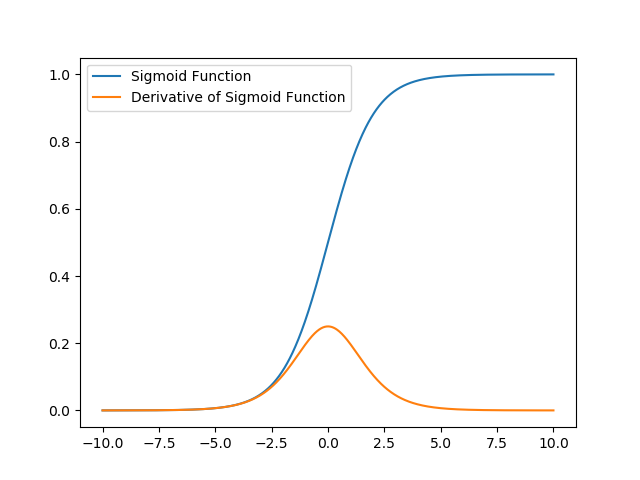
\includegraphics[width=\textwidth]{figures/dl/sigmoid.png}
        \subcaption{Sigmoid Function}\label{fig:Sigmoid}
    \end{subfigure}
    \begin{subfigure}[b]{0.49\textwidth}
        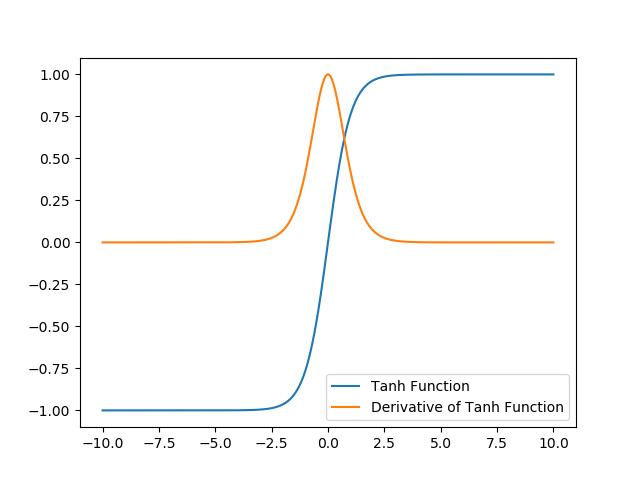
\includegraphics[width=\textwidth]{figures/dl/tanh.png}
        \subcaption{Tanh Function}\label{fig:Tanh}
    \end{subfigure}
    \begin{subfigure}[b]{0.49\textwidth}
        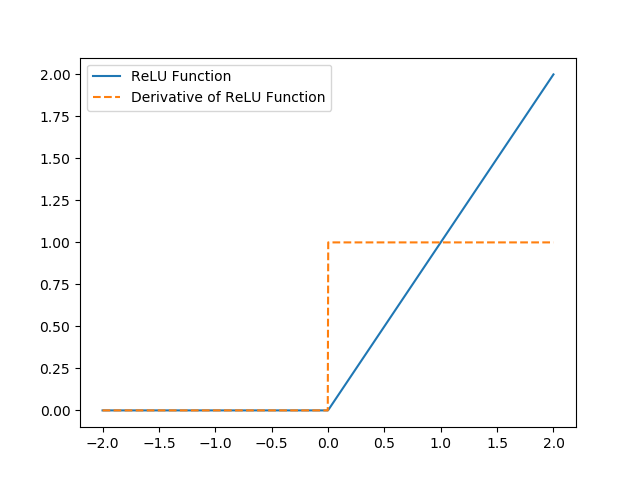
\includegraphics[width=\textwidth]{figures/dl/relu.png}
        \subcaption{ReLU Function}\label{fig:ReLU}
    \end{subfigure}
    \begin{subfigure}[b]{0.49\textwidth}
        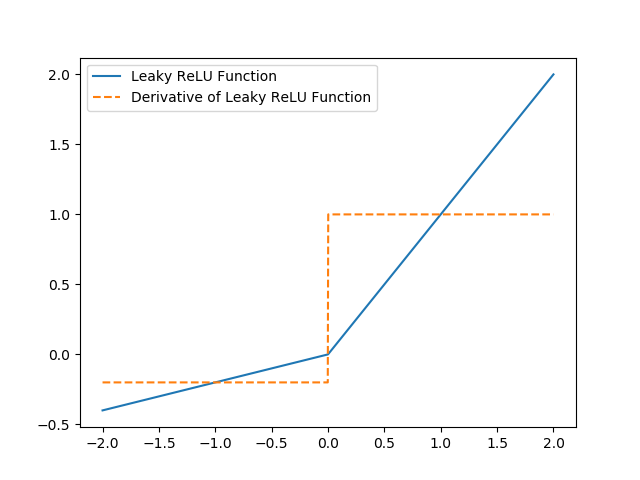
\includegraphics[width=\textwidth]{figures/dl/lrelu.png}
        \subcaption{LeakyReLU Function}\label{fig:LeakyReLU}
    \end{subfigure}
    \caption{Activation Functions}\label{fig:activations}
\end{figure}

\subsection{Sigmoid}
The Sigmoid function, expressed by equation (\ref{eq:sigmoid}) and shown in Figure \ref{fig:Sigmoid} is a logistic function which maps all real values to values within the range of 0 and 1.
A potential issue with the Sigmoid function is that the gradients at all points on the curve are small, with a maximum gradient of just 0.25 where $x = 0$.

\begin{equation}\label{eq:sigmoid}
    \sigma(x) = \frac{1}{1 + e^{-x}}
\end{equation}

\subsection{Tanh}
The Tanh function, expressed by equation (\ref{eq:tanh}) and shown in Figure \ref{fig:Tanh} is related to the Sigmoid function by equation (\ref{eq:sig_tanh})
The Tanh function maps all real values to the range of -1 and 1.
While the Tanh function has stronger gradients than the Sigmoid function, the gradients are still close to zero for most input values of $x$.

\begin{equation}\label{eq:tanh}
    \tanh(x) = \frac{e^x - e^{-x}}{e^x + e^{-x}}
\end{equation}

\begin{equation}\label{eq:sig_tanh}
    \tanh(x) = 2\sigma(2x) - 1
\end{equation}

\subsection{ReLU}
The ReLU function (Figure \ref{fig:ReLU}) is a non-linear function with strong gradient values for all input values of $x$ above zero.
Unlike the Sigmoid and Tanh function, the ReLU function is not differentiable everywhere due to the function not being continuous.
The gradient at the point where $x = 0$ is often treated as zero by library implementations to avoid this issue.

\begin{equation}\label{eq:relu}
    \text{ReLU}(x)=\begin{cases}
      x, & \text{if $x>0$}.\\
      0, & \text{otherwise}.
    \end{cases}
\end{equation}

While the ReLU function has a positive gradient where $x > 0$, the gradient is 0 where $x < 0$.
Another proposed activation function is the LeakyReLU function (Figure \ref{fig:LeakyReLU}) described by equation (\ref{eq:lrelu}) where $l$ is a selected parameter.
The LeakyReLU function multiplies the input value $x$ by some parameter $l$, where $l < 1$, such that $x$ is attenuated.

\begin{equation}\label{eq:lrelu}
    \text{LeakyReLU}(x)=\begin{cases}
      x, & \text{if $x>0$}.\\
      lx, & \text{otherwise}.
    \end{cases}
\end{equation}

\subsection{Softmax} \label{softmax}
The Softmax function is commonly used in classification problems in which a model aims to classify an input value $\bm{x}$ as one of $N$ labels.
The Softmax function, expressed by equation (\ref{eq:softmax}), converts the input $\bm{x}$ into a normalised probability distribution over the $N$ labels, the label with the highest likelihood is interpreted as the model's prediction. 
Such models are commonly trained with the Negative Log Likelihood loss function, by applying the log to the output of the Softmax function.

\begin{equation}\label{eq:softmax}
    \text{Softmax}(x_i) = \frac{e^{x_i}}{\sum_j^N e^{x_j}}
\end{equation}

The Negative Log Likelihood loss function can be expressed by equation \ref{eq:nll} where $\mat{x}$ is the prediction from the Softmax function.

\begin{equation}\label{eq:nll}
    \textit{L}(\mat{x}) = -\log (\mat{x})
\end{equation}

The Softmax function returns a likelihood value for each label, this can be interpreted as the confidence the model has that the input data values corresponds to each label.
The range of the Negative Log Likelihood shown in Figure \ref{fig:nll} shows that when the model confidence in the correct label is high, the Negative Log Likelihood tends to zero, while when the confidence is low for the correct label, the loss tends to infinity.

\begin{figure}[h]
    \centering
        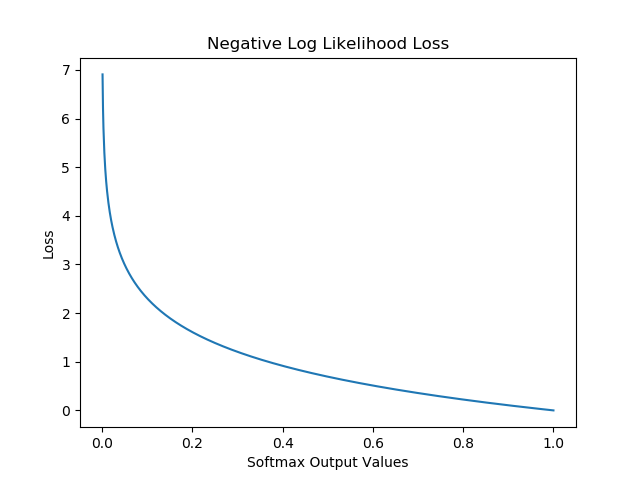
\includegraphics[width=0.7\textwidth]{figures/dl/nll.png}
    \caption{Negative Log Likelihood Loss}\label{fig:nll}
\end{figure}

\section{Optimisation Algorithms}
With the aim of finding the model parameter values which minimise the loss function of the model, Gradient Descent algorithms are commonly used to find such parameters.
Given a loss function $L(x)$ which is to be minimised, where $x$ represents the model parameters, the value of $x$ is iteratively updated by calculating the gradient of $L(x)$ for the current parameters and updating the parameters as described by equation (\ref{eq:gradient_descent}).
$\epsilon$ is the learning rate for the algorithm which determines the step size made at each update.
Too large a step size and the update may overshoot the optimum value (Figure \ref{fig:high_lr}), too small a step size may result in a model which takes an impractical length of time to train or may fail to find a global minimum entirely (Figure \ref{fig:low_rl}). 
It's is often useful in practice to begin with a learning rate which is able to make large steps, then to reduce the learning rate $\epsilon$ as the model trains.

\begin{equation}\label{eq:gradient_descent}
   x^\prime = x - \epsilon \nabla_x L(x)
\end{equation}

\begin{figure}[h]
    \centering
    \begin{subfigure}[b]{0.4\textwidth}
        
\includegraphics[width=\textwidth]{figures/dl/high_lr.jpeg}
        \subcaption{Large Learning Rate}\label{fig:high_lr}
    \end{subfigure}
    \begin{subfigure}[b]{0.49\textwidth}
        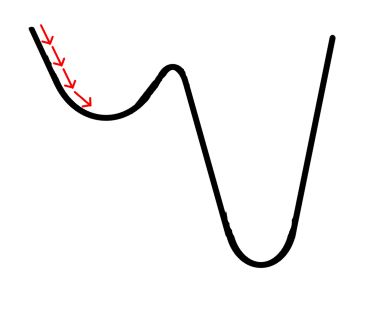
\includegraphics[width=\textwidth]{figures/dl/low_lr.jpeg}
        \subcaption{Small Learning Rate}\label{fig:low_rl}
    \end{subfigure}
    \caption{Learning Rates}\label{fig:learning_rates}
\end{figure}

\subsection{Stochastic Gradient Descent}
Stochastic Gradient Descent (SGD) takes a minibatch of $m$ samples from a data generating independent and identically distributed (i.i.d) distribution, and calculates the average gradient with which the update rule described by equation (\ref{eq:SGD}) is applied.
The use of minibatches results in an approximation of the true gradient as the whole dataset is not evaluated before making an update, just a small subset of the dataset.
This can have the affect of adding regularisation to the learning procedure, particularly with smaller batch sizes \cite{Goodfellow-et-al-2016}.
The SGD update rule for a loss function $L(.)$ and model $f(\bm{x}_i; \bm{\theta})$ can be defined by equation (\ref{eq:SGD}):

\begin{equation*}
    \bm{g} = \frac{1}{m} \nabla_\theta \sum_i^m L(f(\bm{x}_i; \bm{\theta}), y_i)
\end{equation*}

\begin{equation}\label{eq:SGD}
    \bm{\theta}^\prime = \bm{\theta} - \epsilon \bm{g}
\end{equation}

where $\bm{g}$ represents the approximation of the gradient, $\bm{\theta}$ represents model parameters and $\bm{x}_i$ represents $m$ samples making up the minibatch $\{\bm{x}_1, \dots, \bm{x}_m\}$ and corresponding target values $\bm{y}_i$.

\subsection{Momentum}
In order to the accelerate the training of models and find the global minimum faster, momentum is often used with optimisation algorithms.
In addition to the gradient term, a velocity term is also calculated as an accumulation of decaying moving average values from the previous gradient approximation \cite{Goodfellow-et-al-2016}.
The result of this is that the optimisation will continue to move in the direction in which it has been moving, aiding in the prevention of the model becoming stuck in local minimum.
Figure \ref{fig:Momentum} demonstrates how momentum may accelerate the optimisation process.
Here the black arrows represent the gradient evaluated at each point, while the red line shows the path taken with momentum.

\begin{figure}[h]
    \centering
        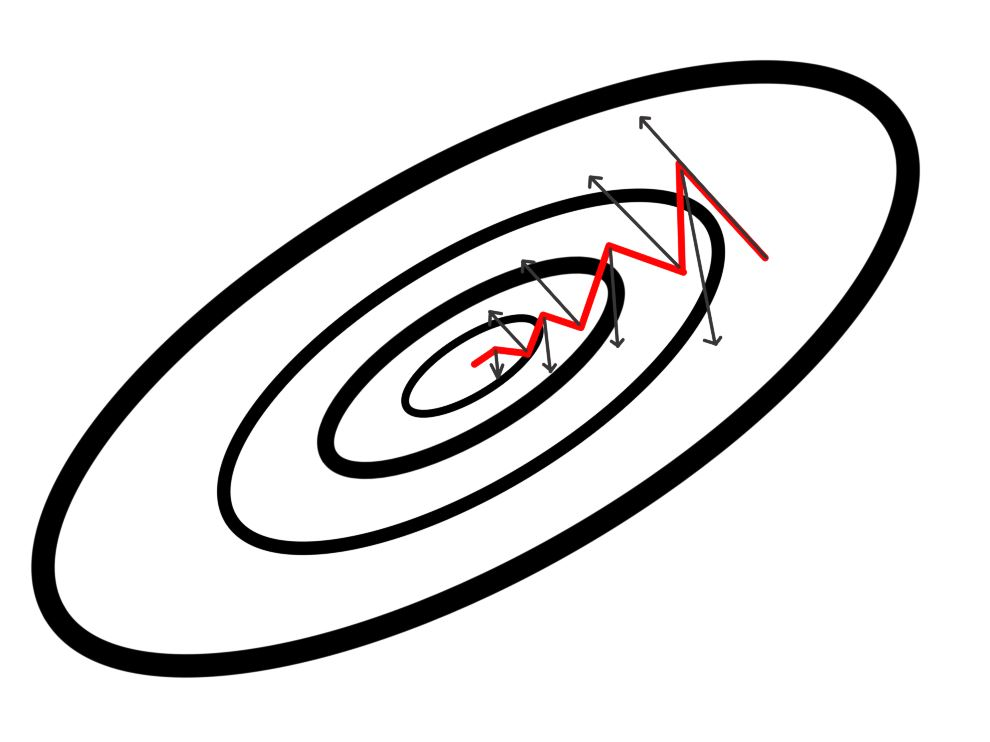
\includegraphics[width=0.6\textwidth]{figures/dl/momentum.jpeg}
    \caption{SGD with Momentum \cite{Goodfellow-et-al-2016}}\label{fig:Momentum}
\end{figure}

\subsubsection{Adaptive Learning Algorithms}
Such algorithms as RMSprop and Adam exist which are built upon the principles of the SGD algorithm with the addition of momentum but adapt their learning rates or momentum values based on a history of previous gradient values.
These aid in finding the global minimum for the loss function at hand.

\subsection{RMSprop}
While momentum can be used to help reduce oscillations while training, RMSprop goes further by updating the learning rate dependent on each dimension in the loss function.
Given a pair of weight parameters $b$ and $w$, during training these are improved to find the optimal solution.
During training the contour plot in Figure \ref{fig:rmsprop} can be seen to oscillating a large amount in the $b$ axis.

\begin{figure}[h]
    \centering
        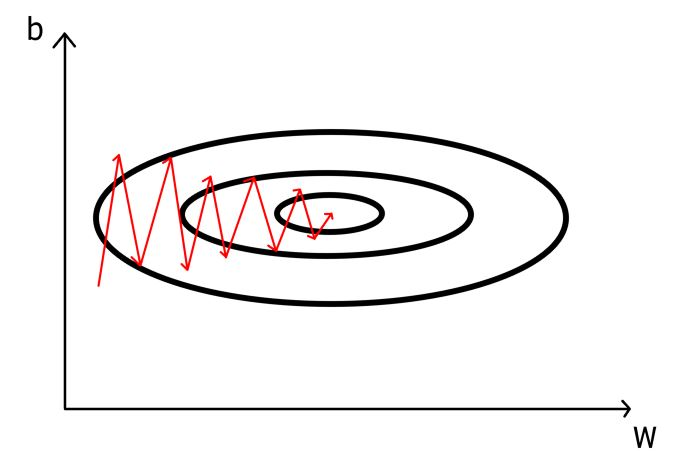
\includegraphics[width=0.7\textwidth]{figures/dl/rmsprop.jpeg}
    \caption{Incentive Behind RMSprop \cite{Goodfellow-et-al-2016}}\label{fig:rmsprop}
\end{figure}

To prevent this oscillation the learning rate could be reduced, but it can also be seen that it would be desirable for the learning rate for the $w$ parameter to be increased as the model would converge faster.
RMSprop is an adaptive learning rate optimisation algorithm which aims to reduce the learning rate for parameters with large gradients and increase the learning rate for those with small gradients \cite{Goodfellow-et-al-2016}. 

This is achieved by keeping an sum of weighted squares of the derivatives of each parameter, where $\beta$ is a tunable hyperparameter:
\begin{equation*}
    \begin{aligned}
        S_{\delta w} &= \beta S_{\delta w} + (1 - \beta) \delta w^2 \\
        S_{\delta b} &= \beta S_{\delta b} + (1 - \beta) \delta b^2
    \end{aligned}
\end{equation*}

The weight parameters are then updated with the root mean square of the weighted sum of the parameter derivative, where $\alpha$ is a tunable hyperparameter.
\begin{equation}\label{eq:rmsprop}
    \begin{aligned}
        w &= w - \alpha \frac{\delta w}{\sqrt{S_{\delta w}}} \\
        b &= b - \alpha \frac{\delta b}{\sqrt{S_{\delta b}}}
    \end{aligned}
\end{equation}

When the gradient of the weight parameter is large, the learning rate for that values is small, while weight parameters with small gradient values are updated with a larger learning rate, as expressed by equation (\ref{eq:rmsprop}).



%%%%%%%%%%%%%%%%%%%%%%%%%%%%%%%%%%%%
\documentclass[12pt]{report}

% some macros
% Here, you can define your own macros. Some examples are given below.

\newcommand{\R}[0]{\mathds{R}} % real numbers
\newcommand{\Z}[0]{\mathds{Z}} % integers
\newcommand{\N}[0]{\mathds{N}} % natural numbers
\newcommand{\C}[0]{\mathds{C}} % complex numbers
\newcommand{\bm}[1]{{\boldsymbol{{#1}}}} % vector
\newcommand{\mat}[1]{{\boldsymbol{{#1}}}} % matrix

\newcommand{\E}[1]{\mathbb{E}_{#1}} % Expectation
\newcommand{\Pd}[1]{\mathbb{P}_{#1}} % Probability Distribution

%%%%%%%%%%%%%%%%%%%%%%%%%%%%%%%%%%%%%%%%%
% University Assignment Title Page 
% LaTeX Template
% Version 1.0 (27/12/12)
%
% This template has been downloaded from:
%%%%%%%%%%%%%%%%%%%%%%%%%%%%%%%%%%%%%%%%%
%----------------------------------------------------------------------------------------
%	PACKAGES AND OTHER DOCUMENT CONFIGURATIONS
%----------------------------------------------------------------------------------------

\usepackage[nottoc,notlot,notlof]{tocbibind}
\usepackage[T1]{fontenc}
%\usepackage{hyperref}
\usepackage{indentfirst}
\usepackage{amsmath}
\usepackage{amssymb}
\usepackage{graphicx}
\usepackage{subcaption}
\usepackage{geometry}
 \geometry
 {
     a4paper,
     left=25mm,
     right=25mm,
     top=30mm,
     bottom=30mm,
 }

% \usepackage[a4paper,hmargin=2.8cm,vmargin=2.0cm,includeheadfoot]{geometry}
\usepackage{textpos}
\usepackage{natbib} % for bibliography
%\usepackage{tabularx,longtable,multirow,subfigure,caption}
\usepackage{fncylab} %formatting of labels
\usepackage{fancyhdr} % page layout
\usepackage{url} % URLs
\usepackage[english]{babel}
%\usepackage{dsfont}
\usepackage{epstopdf}
\usepackage{backref} % needed for citations
\usepackage{array}
\usepackage{latexsym}
\usepackage[pdftex,pagebackref,hypertexnames=false,colorlinks]{hyperref} % provide links in pdf
 
\hypersetup{pdftitle={},
  pdfsubject={}, 
  pdfauthor={},
  pdfkeywords={}, 
  pdfstartview=FitH,
  pdfpagemode={UseOutlines},% None, FullScreen, UseOutlines
  bookmarksnumbered=true, bookmarksopen=true, colorlinks,
    citecolor=black,%
    filecolor=black,%
    linkcolor=black,%
    urlcolor=black}
 
\usepackage[all]{hypcap}
\frenchspacing

\DeclareMathOperator{\tr}{tr}

\begin{document}

\chapter{Literature Review}

TO-DO
Add introduction to lit review

\section{Current Lip Reading Models and Datasets}

In recent years the problem of visual speech recognition (VSR), also know as lip reading, has seen huge advances due to the availability of new datasets and the use of Deep Learning models \cite{Chung2016, Chung2017, Shillingford2018}.
This section shall discuss the progresses which have already been made in this field and the datasets publicly available on which to train such models.
Current lip reading models, to the best of the author's knowledge, all make use of 2D temporal data such as videos by evaluating the frames of the video, using this information to make a prediction of the word, or words, which were spoken in the sequence.

However in reality, humans who are able to lip read also have access to three dimensional data due to our depth perception, which is not well represented in 2D video frames; thus is can be hypothesised that some information captured by 3D temporal scans of speaking subjects can also be used for speech prediction.
Unlike 2D temporal data, 3D temporal data (3D video), requires multiple cameras to record simultaneously, which in turn requires synchronisation between the cameras, increasing the complexity of the system beyond simply having multiple cameras.
The data must then be processed to produce the final product, whether this is in the form of video with depth information or more complex 3D scans \cite{Li2017}.

\subsection{Datasets}
There currently exists multiple labelled video datasets which can be used for traditional VSR; here 'traditional' refers to using 2D temporal data.
Datasets such as GRID \cite{Cooke2006}, LRW \cite{Chung2016}, LRS \cite{Chung2017} and LSVSR \cite{Shillingford2018} have been constructed by compiling the video data from various sources, each with an increasing vocabulary and dataset size.

\subsubsection{Controlled Conditions Datasets}
The GRID dataset was released in 2006 \cite{Cooke2006} and contains 34,000 samples from 34 speakers, each with 1000 sentences.
Based on previous work using the coordinate response measure (CRM) \cite{Bolia2000}, the corpus uses sentences with a fixed grammar: <command:4>, <colour:4>, <preposition:4>, <letter:25>, <number:10>, <adverb:4>, with a total vocabulary of 51 words.
Aside from the restricted vocabulary size in comparison to more recent datasets, the primary limiting factor of the GRID dataset is that all data was captured directly for the use of the dataset and so, models trained on this dataset have learnt on controlled conditions, something not found in the desired wider applications of VSR.

\subsubsection{In The Wild Datasets}
To build larger datasets more suited for deep learning models, the following are commonly built with "in the wild" data, meaning that the original videos have not been captured with the intention of being used for this dataset, while the data collected for the datasets is preprocessed such that it is suited for the task.
Variations in lighting, angles, speakers and a wide vocabulary are common, this does however make the datasets more challenging to learn from, but the models are no longer as bias to controlled conditions.

LRW and LRS are both comprised of content from BBC broadcasts \cite{Chung2016, Chung2017} allowing for a far larger corpus size of 500 words for LRW and over 6000 words for LRS.
Both of datasets are captured and processed with the same pipeline (Figure \ref{fig:LRW_Pipeline}) summarised as follows. 

\begin{figure}[h]
    \centering
        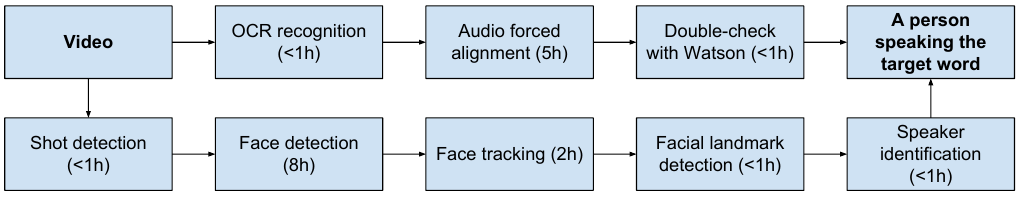
\includegraphics[width=0.8\textwidth]{figures/lrw_pipeline.png}
    \caption{LRW Dataset Pipeline \cite{Chung2016}}\label{fig:LRW_Pipeline}
\end{figure}

Firstly, as the text transcripts are broadcast as bitmaps, optical character recognition (OCR) \cite{Buehler2009} is used to obtain the text spoken in the video, the audio and text are then aligned per frame using the HTK toolkit \cite{Woodland1995}.
The quality of these predictions are validated with the use of the commercial IBM Watson Speech to Text converter.

Secondly, face detection and tracking are used so that the frame can be cropped to feature the subject's mouth at the centre.
To achieve this, a histogram of oriented gradients based (HOG-based) detection algorithm \cite{King2009} is used on all video frames to detect faces, see left hand side of Figure \ref{fig:LRW_Face_Detection}.
A Kanade-Lucas-Tomasi (KLT) feature tracker is also applied to the frames, where both the HOG and KLT overlap (see centre of Figure \ref{fig:LRW_Face_Detection}), it is assumed to be tracking the face correctly.
To identify mouth position, facial landmarks are then used using an ensemble of regression trees method from \cite{Kazemi2014}, see the right of Figure \ref{fig:LRW_Face_Detection}.
As multiple faces can appear at any one time, it is assumed that the speaker will be the only subject with a moving mouth.
Assuming that the lip movements fall within a frequency range, the Fourier transform is applied to the openness of the mouth defined by the distance between top and bottom lip from the facial landmarks.
A support vector machine (SVM) is then trained on the frequency spectrum to classify who is speaking in each frame.
The frames are then cropped around the relevant speaker.

\begin{figure}[h]
    \centering
        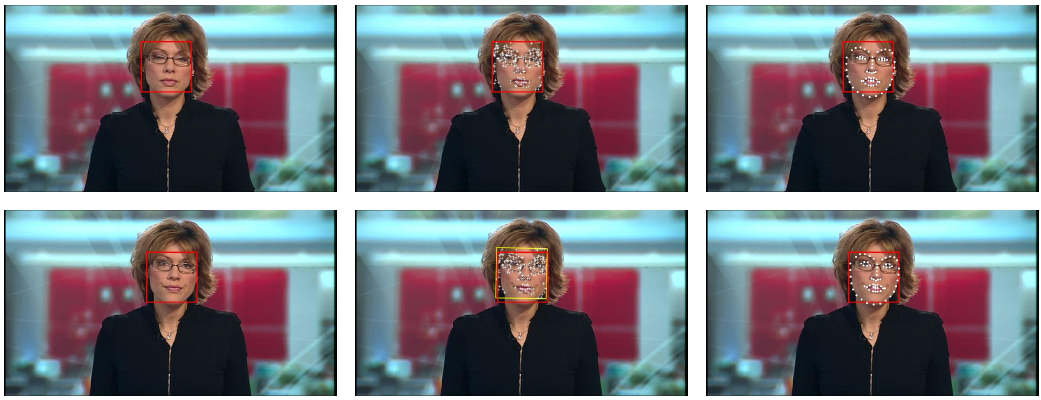
\includegraphics[width=0.8\textwidth]{figures/lrw_face_detection.png}
    \caption{LRW Face Detection and Tracking \cite{Chung2016}}\label{fig:LRW_Face_Detection}
\end{figure}

LSVSR is a dataset published by DeepMind and Google which makes use of the huge amount of videos on YouTube \cite{Shillingford2018}, resulting in a total length of 3886 hours of training data.
Unlike LRW or LRS, LSVSR aligns phonemes to frames, as opposed to words or characters.
The pre-processing steps are similar as in LRW and LRS, although the alignment is performed with the algorithm laid out in previous work by DeepMind \cite{Liao2013}.

\subsubsection{3D Datasets} \label{3D Datasets}
To the best of the author's knowledge, there are currently only two datasets with 3D temporal data which could be appropriate for training lip reading models, neither of which have been captured with the intention of being used for VSR.

The first of which is LRW-3D \cite{Tzirakis2019} which has been captured from four subjects, two native English speakers and two non-native to increase variability in the dataset.
The subjects have been captured speaking the corpus used in the LRW dataset \cite{Chung2016}, a vocabulary of 500 words.
The resulting dataset comprises of 660 seconds of 3D meshes and audio per subject.
The dataset is not comprised of full sentences but would be appropriate for word-level lip reading, however a total duration of 660 seconds is likely to be too short for a deep learning model to train effectively.
The dataset had also not been officially published at the time of this report.

The second is the VOCASET \cite{Cudeiro2019}, an unlabelled dataset captured from 6 male and 6 female subjects.
Each subject was recorded speaking 40 sequences, each ranging from 3 to 5 seconds, resulting in a total time of 30 minutes.
The recorded 3D meshes are registered to the FLAME model \cite{Li2017}, a statistical 3D facial mesh with around 5000 vertices.
Unlike the LRW-3D dataset, the sequences are grammatically correct sentences, chosen to maximise phonetic diversity.
This makes the VOCASET appropriate for creating a model for sentence-level lip reading, similarly to LRW-3D, 30 minutes of training data is likely to be a limiting factor when training a deep learning model.

It should be noted that neither of these datasets were captured for the purpose of lip reading, but for synthesising realistic statistical facial models driven from an audio input, and thus there are no transcriptions for VOCASET.
The transcriptions can be obtained with an Audio Speech Recognition (ASR) method such as DeepSpeech \cite{Hannun2014} and then alignment would have to be performed to the datasets before using the data to train lip reading models.

\subsection{Lip Reading Models}
Chung et al \cite{Chung2016} used a convolutional model based on the VGG-M architecture which produced character level distributions with the LRW dataset, these distributions are then processed by a language model for text prediction.

The LipNet model \cite{Assael2016} was produced to be able to predict sentence-level lip reading of varied length, while previous work by \cite{Chung2016} predicted on a word level.
The model used spatiotemporal convolutions to process multiple frames of video at once followed by a recurrent layer using Gated Recurrent Units (GRU) \cite{Cho2014}.
The model used the GRID dataset \cite{Cooke2006} in which all subjects are recorded under consistent conditions of good lighting and fixed angles.
LipNet achieved the state of the art performance on the GRID dataset by using an model with increased complexity by incorporating 3D convolution and recurrent units.

As the LRW dataset could not be used to train a model such as LipNet for sentence-level lip reading, but the GRID dataset had limitations in the number of subjects and vocabulary, Chung et al created the LRS dataset \cite{Chung2017}.
The model presented was trained on both audio and video and made capable of taking either or both as the model inputs.
To prevent the model from being dependent on a single input source, the inputs are systematically distorted or removed.
The video input is passed through convolutional layers, followed by LSTM layers, while the audio is converted to Mel-frequency cepstral coefficients (MFCC), then input to LSTM layers.
The two are combined with then attention mechanism and further LSTM layers and an output fully connected layer with softmax activation for character distributions.
The model also makes use of curriculum learning by initially training the model on short sequences of single words.
The length of training sequences are increased throughout training.
It is stated by \cite{Chung2017} that this accelerates training and reduces overfitting.

In 2018 DeepMind published their V2P model \cite{Shillingford2018} along with the LSVSR dataset which is larger than all previous datasets, containing 3886 hours of training data.
The model follows a similar architecture to LipNet \cite{Assael2016} but with an increased number of convolutional layers and LSTM layers rather than GRUs.
It should be commented that due to the size of the model and dataset dictated the use of 64 GPUs for training to allow a batch size of 128.
Unlike previous models, the V2P model predicts phonemes as opposed to characters, these phonemes are then processed by a language model for word prediction as with previous models.

To the best of the author's knowledge, currently there do not exist any papers which have explored the use of 3D temporal datasets for the use with lip reading models. 
This is likely due to the shortage of 3D temporal data due to the difficulties in obtaining such data, on which such models could be trained on.

\section{Data Generation}
In order to construct a deep learning lip reading model capable of being trained on 3D temporal data, appropriate datasets must be established.
Current datasets have been captured directly \cite{Tzirakis2019, Cudeiro2019} with the use of multi-camera capture rigs under controlled situations.
The total duration of both of these datasets is very short in comparison to the video datasets such as LRW, LRS and LSVSR, which is a limiting factor as to the models which could be trained using them.

As the models also use different mesh models to represent the data that has been captured this also prevents the two datasets being joined directly.
Unlike video data, there currently lacks a large body of 3D video data which is publicly available, limiting the construction of 3D datasets to directly capturing more 3D scans with multi-camera capture rigs, similar to those used in \cite{Tzirakis2019, Cudeiro2019} and generating synthetic training data.

\subsection{Audio Driven Data Generation}
Karras et al proposed a method for generating 3D facial animation from audio with the use of a CNN architecture \cite{Karras2017a}.
The model is actor specific, but is only trained on 3-5 minutes of data of the actor.
Short range temporal features are first extracted from the audio by a formant analysis network.
This representation is then analysed by an articulation network which also accepts a learned emotional state of the speaker.
The output layer drives displacements from a neutral 3d mesh of the actor.

However, as the model by Karras et al. is not independent of the actor it cannot generalise to new subjects.
Tzirakis et al. propose a model which is independent of speaker and capture rig \cite{Tzirakis2019}.
As discussed in section \ref{3D Datasets}, a dataset was constructed of 3D speaking faces using the LRW dataset \cite{Chung2016} for the corpus.
This allowed Tzirakis et al. to create a model which can synthesise facial motion from audio from the LRW dataset.
The model used is similar to that used in \cite{Karras2017a}, firstly extracting short term temporal features from the input audio with a convolutional network followed by another convolutional network to analyse the extracted features.
Unlike the model used in \cite{Karras2017a}, the model used in \cite{Tzirakis2019} is trained to drive learnt blendshapes.
This reduces the number of output parameters of the model substantially in comparison to that used by Karras et al.

Similar to \cite{Tzirakis2019}, the VOCA model \cite{Cudeiro2019} synthesises video sequences of 3D models speaking given an audio input.
The VOCASET dataset discussed in section \ref{3D Datasets}, was captured with the intention of training this model to be independent of the speaker, hence a large range of speakers are used within the dataset.
The model is comprised of three sections: audio feature extraction, a feature encoder and a decoder to drive a template facial mesh from the FLAME model \cite{Li2017}.
The audio feature extraction makes use of the pre-trained Mozilla implementation of the DeepSpeech model, based on the paper by Hannun et al. \cite{Hannun2014}.
The DeepSpeech model takes audio as an input and returns the unnormalised log-probabilities for an alphabet of the 26 standard characters, a space, apostrophe and blank character for time slices in the audio input.
The encoder is a convolutional network which is conditioned on the speakers identity, such that the latent space of speaker styles can later be explored on new audio inputs.
Finally, the decoder is made up of a fully connected layer with a linear activation function is used to output the displacements of the 5023 vertices in the template face.

\bibliographystyle{unsrt}
\bibliography{ref}
\end{document}


%%%%%%%%%%%%%%%%%%%%%%%%%%%%%%%%%%%%
%\documentclass[12pt]{report}
%
%% some macros
%% Here, you can define your own macros. Some examples are given below.

\newcommand{\R}[0]{\mathds{R}} % real numbers
\newcommand{\Z}[0]{\mathds{Z}} % integers
\newcommand{\N}[0]{\mathds{N}} % natural numbers
\newcommand{\C}[0]{\mathds{C}} % complex numbers
\newcommand{\bm}[1]{{\boldsymbol{{#1}}}} % vector
\newcommand{\mat}[1]{{\boldsymbol{{#1}}}} % matrix

\newcommand{\E}[1]{\mathbb{E}_{#1}} % Expectation
\newcommand{\Pd}[1]{\mathbb{P}_{#1}} % Probability Distribution

%%%%%%%%%%%%%%%%%%%%%%%%%%%%%%%%%%%%%%%%%%
% University Assignment Title Page 
% LaTeX Template
% Version 1.0 (27/12/12)
%
% This template has been downloaded from:
%%%%%%%%%%%%%%%%%%%%%%%%%%%%%%%%%%%%%%%%%
%----------------------------------------------------------------------------------------
%	PACKAGES AND OTHER DOCUMENT CONFIGURATIONS
%----------------------------------------------------------------------------------------

\usepackage[nottoc,notlot,notlof]{tocbibind}
\usepackage[T1]{fontenc}
%\usepackage{hyperref}
\usepackage{indentfirst}
\usepackage{amsmath}
\usepackage{amssymb}
\usepackage{graphicx}
\usepackage{subcaption}
\usepackage{geometry}
 \geometry
 {
     a4paper,
     left=25mm,
     right=25mm,
     top=30mm,
     bottom=30mm,
 }

% \usepackage[a4paper,hmargin=2.8cm,vmargin=2.0cm,includeheadfoot]{geometry}
\usepackage{textpos}
\usepackage{natbib} % for bibliography
%\usepackage{tabularx,longtable,multirow,subfigure,caption}
\usepackage{fncylab} %formatting of labels
\usepackage{fancyhdr} % page layout
\usepackage{url} % URLs
\usepackage[english]{babel}
%\usepackage{dsfont}
\usepackage{epstopdf}
\usepackage{backref} % needed for citations
\usepackage{array}
\usepackage{latexsym}
\usepackage[pdftex,pagebackref,hypertexnames=false,colorlinks]{hyperref} % provide links in pdf
 
\hypersetup{pdftitle={},
  pdfsubject={}, 
  pdfauthor={},
  pdfkeywords={}, 
  pdfstartview=FitH,
  pdfpagemode={UseOutlines},% None, FullScreen, UseOutlines
  bookmarksnumbered=true, bookmarksopen=true, colorlinks,
    citecolor=black,%
    filecolor=black,%
    linkcolor=black,%
    urlcolor=black}
 
\usepackage[all]{hypcap}
\frenchspacing

\DeclareMathOperator{\tr}{tr}
%
%\begin{document}

\externaldocument{lit_review}
\externaldocument{facial_modelling_background}
\externaldocument{appendix}

\chapter{Blendshape Classification}

This chapter shall discuss the problem of word level classification from blendshape parameters obtained from a dataset created with the VOCA model \cite{Cudeiro2019} processing audio from the LRW dataset \cite{Chung2016}.
Classification is performed with a Convolutional Neural Network architecture on 500 labels.
The model architecture, how performance is assessed and how the model has been tuned to maximise performance on a held out validation set is also discussed. 

\section{Problem Definition}
As with traditional lip reading problems, the end goal of VSR models using 3D temporal data is to correctly classify variable length input sequences at a sentence level.
However, before this problem can be tackled, the simpler problem of word level classification should be first approached to ensure that this is possible, before moving on to more advanced problems.
If word level classification cannot be achieved, it may be concluded that there is not a sufficient amount of information encoded in 3D temporal models for more complex problems to be solved with the current set of assumptions.

These assumptions include:
\begin{enumerate}
    \item Provided an appropriate dataset of 3D temporal facial scans of subjects speaking, a set of blendshape parameters which realistically represent the motions of speech can be found. \label{assumption:class_1}
    \item The blendshape parameters represent an encoding from which a classification model is able to make word level predictions. \label{assumption:class_2}
\end{enumerate}

\section{Generation of a 3D Lip Reading Dataset}
In order to train any model, an appropriate dataset must exist upon which the model can be trained.
An appropriate dataset for word level prediction from blendshape parameters would consist of:
\begin{itemize}
   \item A large enough vocabulary that single instances of words with unique phonemes do not exist, as this would allow classification of these words to be too simple.
   \item Facial mesh recordings for all samples in the dataset, all of which brought into alignment to remove movement not related to speech.
   \item Principal blendshape axis which can be shown to contain useful interpolation for speech.
   \item The blendshape parameters corresponding to each sample for the given blendshape axis.
\end{itemize}

As discussed in section \ref{3D Datasets}, currently there exists no public datasets which have been created for the purpose of lip reading from 3D temporal data.
In addition to this, the datasets which have not been created with the purpose of lip reading but do contain 3D temporal data of speaking facial scans, are either not public in the case of Karras's model \cite{Karras2017a} or are unlabelled and too small to train a model effectively as is the case with the VOCASET \cite{Cudeiro2019}.
Both of these datasets also contain a large vocabulary, with too few samples of each word.
The VOCASET dataset could be labelled with the use of an automatic speech recognition model such as DeepSpeech as suggested in section \ref{3D Datasets}, however as the dataset was constructed to contain as much variation in speech sounds, so a degree of word repetition would offer little benefit, hence the lack of consistent word repetition.

In order to tackle the issue of an appropriate dataset not existing, two solutions exist.
The ideal solution would be to capture subjects speaking words from a set corpus using a 3D capture equipment, this solution was not a viable option for this project due to the specialised equipment required and the data processing required after data capture had been performed.
Another means of constructing the dataset would be to generate the data with an existing model which can convert an appropriate audio dataset to a series of facial meshes from which blendshape axis can be constructed and parameters recovered.
This can be achieved by processing audio from the LRW dataset \cite{Chung2016} though the VOCA model \cite{Cudeiro2019}.
The VOCA model claims to be able to generate realistic 3D facial motion from audio, as lip reading is notoriously difficult for humans, this is difficult to validate.
Assuming that the VOCA model does in fact generate realistic facial motion, the LRW dataset allows for a 3D dataset to be generated with a set corpus of the 500 words contained in the LRW dataset.

55,000 audio samples are taken from the LRW dataset with a uniform distribution of all labels, resulting in 110 samples for each label.
Audio samples from the LRW dataset are from ``in the wild'' scenarios \cite{Chung2016}, meaning that there is background noise and audio in the clip.
An sample of the word ``\textit{ABOUT}'' will contain the word ``\textit{ABOUT}'' within the audio sample, but will contain other speech either side of the clip.
Figure \ref{fig:LRW_About} shows such a sample labelled as ``\textit{ABOUT}'' in which the phrase ``talking about fair'' is spoken.

\begin{figure}[h]
    \centering
        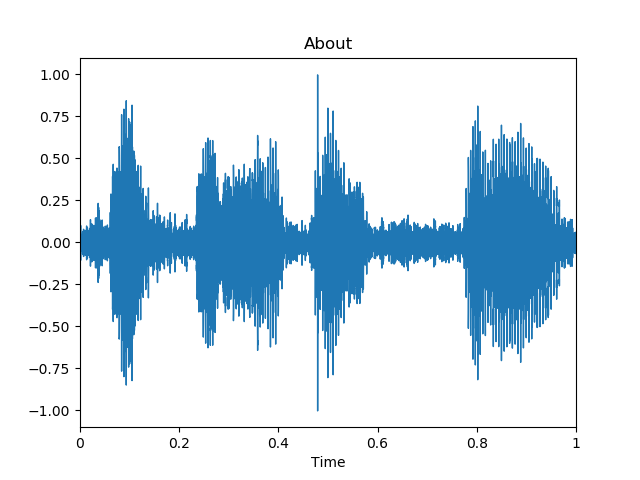
\includegraphics[width=0.7\textwidth]{figures/dataset/about.png}
    \caption{Audio Sample from LRW \cite{Chung2016} ``Talking About Fair''}\label{fig:LRW_About}
\end{figure}

The full LRW dataset contains 1000 training samples for each label, however due to the size of the VOCA model, processing 55000 samples (11\% of the full dataset) took roughly 8 days to process with the GPU acceleration of an Nvidia Tesla M60.
This is due to the size of the VOCA model, which incorporates the DeepSpeech model as a means of audio feature extraction.
In parallel to the generation of the 3D temporal data from the VOCA model, blendshape parameters were recovered as the facial scans were produced.
No significant decrease in the speed of data generation was observed running these tasks in parallel.

\subsection{Blendshape Axis Creation}
Ideally, all 55000 samples would be collected and the PCA would be performed on this to construct the blendshape axis.
However, due to disk space limitations a complete dataset of 55000 facial scans could not be collected at once due to the size of the generated facial meshes as this would total 2.365 million generated facial mesh data samples, each of which occupying around 185KB, requiring a total of 440GB of disc space.
To perform PCA on the generated facial meshes for blendshape axis (see section \ref{blendshapes}), the first 5000 facial mesh sequences were generated totalling 83 minutes of data and 215000 individual facial mesh data samples. 
Once PCA has been applied to a dataset of facial scans, the transformation matrix $\mat{W}$ is known.
$\mat{W}$ has columns of eigenvectors corresponding to eigenvalues, each of these eigenvectors represents the principal axis upon which can be interpolated.
These axes are the blendshapes axes and by interpolating along these axes by given amounts, motions of the facial mesh can be expressed in a low dimension.
The first blendshape axis corresponds to the largest eigenvalue, as that axis contains the largest amount of variation amongst the dataset.
The number of blendshapes which can be created will be limited by the number of positive non-zero eigenvalues found from PCA, however as each successive blendshape axis corresponds to a decreasingly small eigenvalue, the amount of variation in each successive axis decreases. 
This results in realistic reconstruction being able to be achieved with a relatively small number of blendshapes containing the majority of the variation within the dataset.
Examples of the First and Second Blendshape Axis from the first 5000 samples are shown in Figures \ref{fig:Blendshape_axis_1} and \ref{fig:Blendshape_axis_2} respectively, further examples can be viewed in the Appendix: Figure \ref{fig:Blendshape_axis_3}, \ref{fig:Blendshape_axis_4}.
These are constructed by interpolating along each axis individually by a fixed step amount.

\begin{figure}[h]
    \centering
    \begin{subfigure}[b]{0.24\textwidth}
        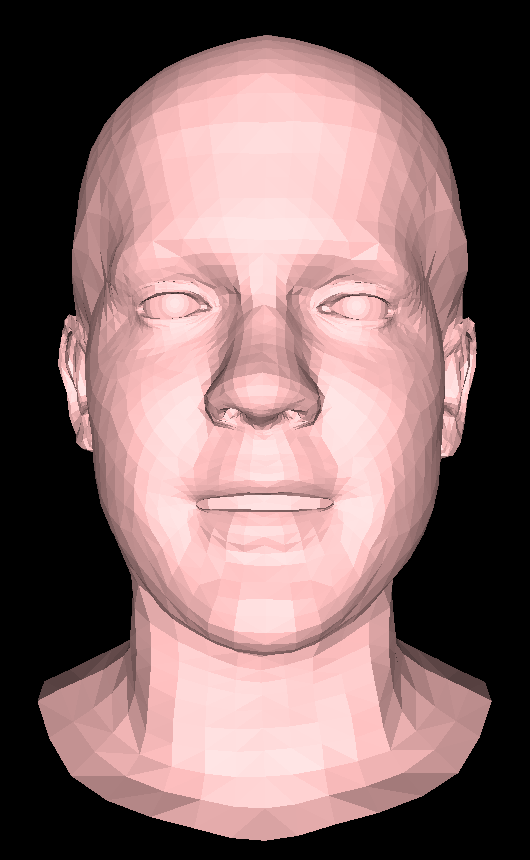
\includegraphics[width=\textwidth]{figures/blendshape_interp/1/00001.png}
    \end{subfigure}
    \begin{subfigure}[b]{0.24\textwidth}
        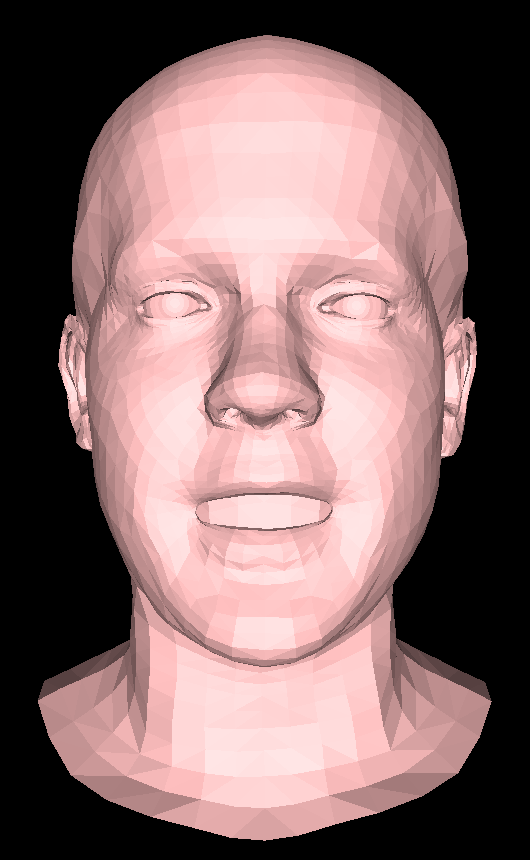
\includegraphics[width=\textwidth]{figures/blendshape_interp/1/00002.png}
    \end{subfigure}
    \begin{subfigure}[b]{0.24\textwidth}
        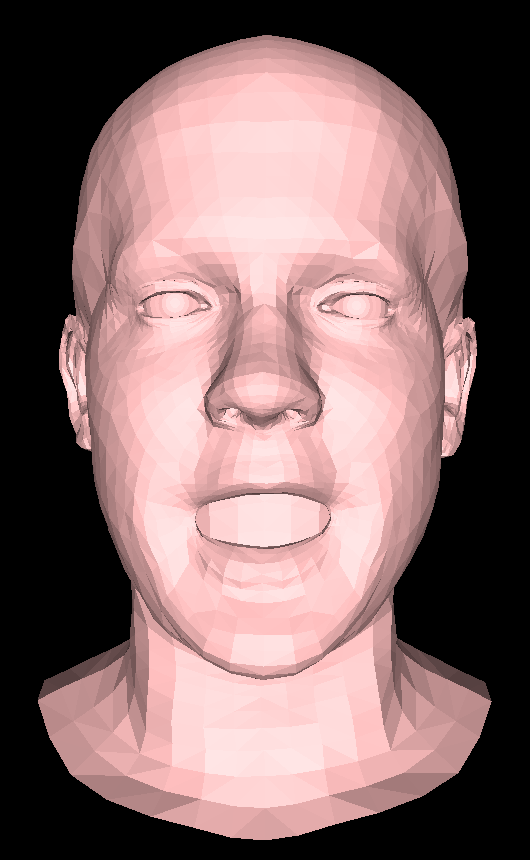
\includegraphics[width=\textwidth]{figures/blendshape_interp/1/00003.png}
    \end{subfigure}
    \begin{subfigure}[b]{0.24\textwidth}
        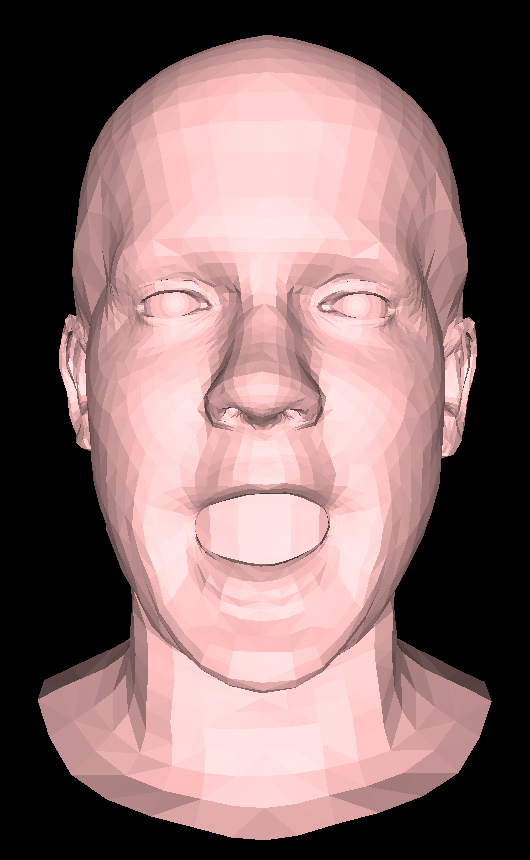
\includegraphics[width=\textwidth]{figures/blendshape_interp/1/00004.png}
    \end{subfigure}
    \caption{First Blendshape Axis Interpolation }\label{fig:Blendshape_axis_1}
\end{figure}
\begin{figure}[h]
    \centering
    \begin{subfigure}[b]{0.24\textwidth}
        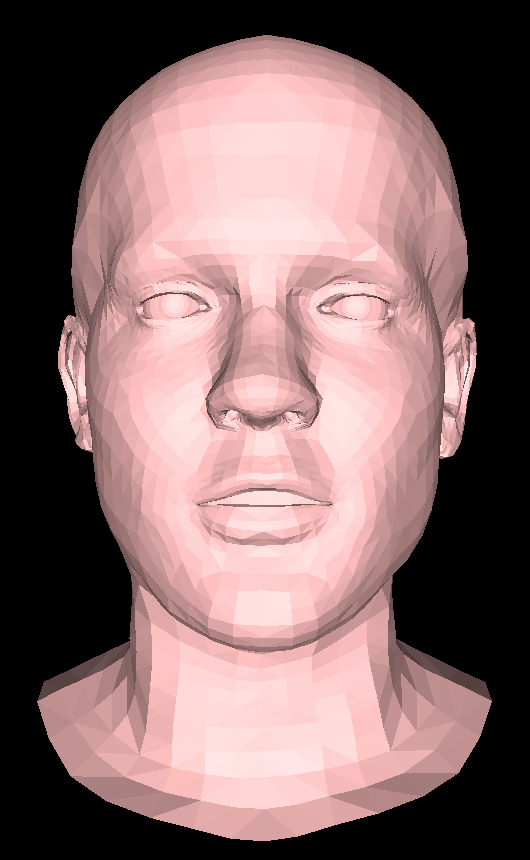
\includegraphics[width=\textwidth]{figures/blendshape_interp/2/00001.png}
    \end{subfigure}
    \begin{subfigure}[b]{0.24\textwidth}
        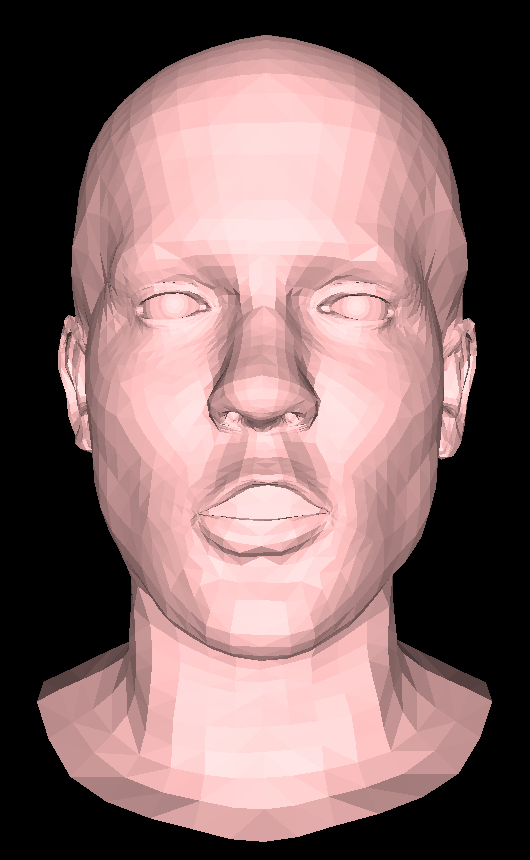
\includegraphics[width=\textwidth]{figures/blendshape_interp/2/00002.png}
    \end{subfigure}
    \begin{subfigure}[b]{0.24\textwidth}
        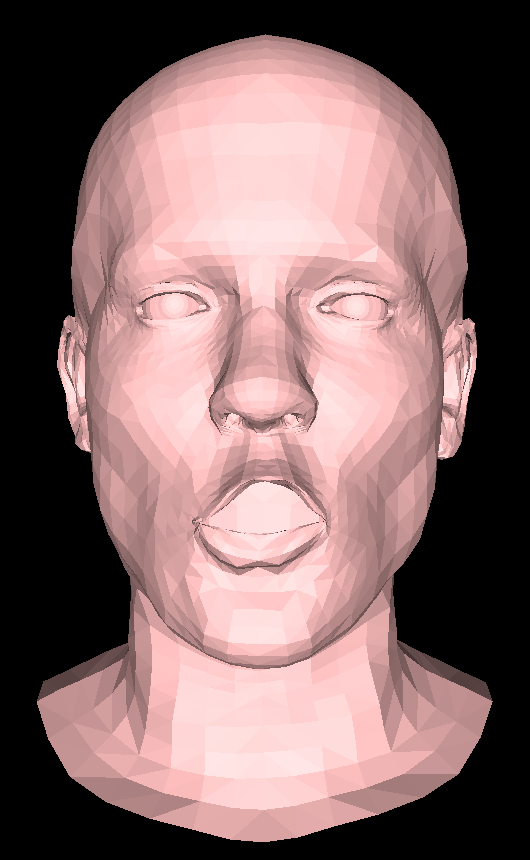
\includegraphics[width=\textwidth]{figures/blendshape_interp/2/00003.png}
    \end{subfigure}
    \begin{subfigure}[b]{0.24\textwidth}
        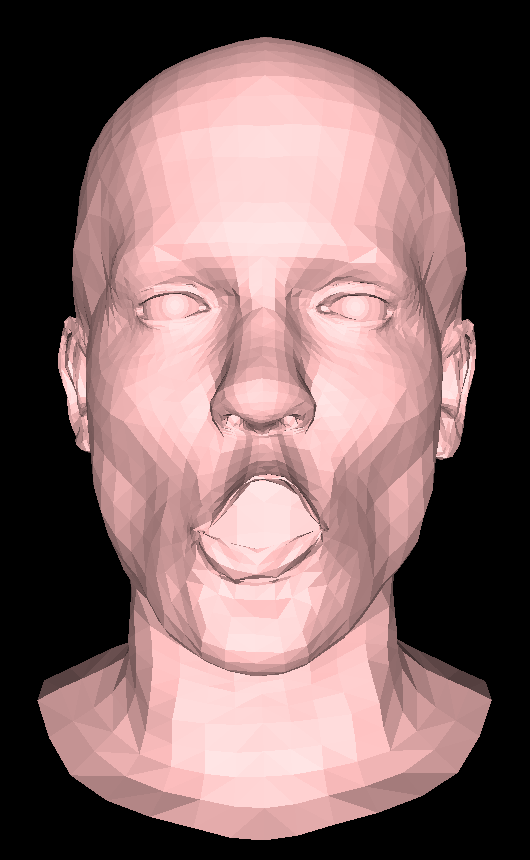
\includegraphics[width=\textwidth]{figures/blendshape_interp/2/00004.png}
    \end{subfigure}
    \caption{Second Blendshape Axis Interpolation}\label{fig:Blendshape_axis_2}
\end{figure}

\subsection{Blendshape Parameter Recovery} \label{sec:blendshape_recovery}
Given a template mesh $\mat{M} \in \mathbb{R}^{(N \times 1)}$ upon which to interpolate, where $N = 3n$ and $n$ represents the number of vertex points in the facial mesh, each of which have an $x, y$ and $z$ coordinate value and Blendshape Axis $\mat{W} \in \mathbb{R}^{(N \times d)}$ as described in section \ref{sec:pca}, where the $d$ first principal axis have been kept, representing the axis along which the template mesh $\mat{M}$ can be interpolated.

\begin{equation*}
    \mat{M} = \begin{bmatrix} 
                x_{1}, &
                y_{1}, &
                z_{1}, &
                \dots, &
                x_{n}, &
                y_{n}, &
                z_{n}
               \end{bmatrix}^\top,
    \quad
    \mat{M} \in \mathbb{R}^{N\times 1},
    \quad
    N = 3n,
\end{equation*}
\quad
\begin{equation*}
    \mat{W} = [
               \bm{w_1}, \dots, \bm{w_d}
              ],
    \quad
    \mat{W} \in \mathbb{R}^{(N \times d)}
\end{equation*}
\quad
\begin{equation*}
    \bm{w_i} = \begin{bmatrix} 
                x_{1}, &
                y_{1}, &
                z_{1}, &
                \dots, &
                x_{n}, &
                y_{n}, &
                z_{n}
    \end{bmatrix}^\top
\end{equation*}

Given subsequent frames $\mat{M}^{\prime}$ which deviate the facial mesh from $\mat{M}$, $\mat{M}^{\prime}$ can be expressed by equation \ref{eq:mesh_interp}, where $\bm{\Lambda}$ is a vector containing Blendshape parameters.

\begin{equation}\label{eq:mesh_interp}
    \mat{M}^{\prime} = \mat{M} + \mat{W} \mat{\Lambda}
\end{equation}
\quad
\begin{equation*}
    \mat{\Lambda} = \begin{bmatrix}
        \lambda_1, &
        \dots, &
        \lambda_d
    \end{bmatrix}^\top
\end{equation*}

The blendshape parameters $\lambda_i$ can be found by rearranging equation (\ref{eq:mesh_interp}) and solving for $\bm{\Lambda}$ as shown in equation (\ref{eq:mesh_interp_lambda}).
The solution to this can be found by finding the pseudo-inverse for the Blendshape Axes $\mat{W}$.

\begin{equation}\label{eq:mesh_interp_lambda}
    \mat{\Lambda} = \mat{W}^{-1}(\mat{M}^{\prime} - \mat{M})
\end{equation}

\section{Data Preprocessing}
To aid training, the dataset is normalised to a range of [0,1] using equation (\ref{eq:normalise}) where $x_{min}$ and $x_{max}$ are the smallest and largest values in the dataset respectively (Figure \ref{fig:hist_norm}).
While each Blendshape Axis is separate from one another, normalisation should be performed on all parameters as a whole to preserve information on the variation found in each Blendshape Axis relative to one another.
As described by PCA in section \ref{sec:pca}, the variation in each subsequent principal axis decreases which can be seen in Figure \ref{fig:hist_norm}.

\begin{equation} \label{eq:normalise}
   x^\prime = \frac{x - x_{min}}{x_{max} - x_{min}} 
\end{equation}

\begin{figure}[h!]
    \centering
    \begin{subfigure}[b]{0.49\textwidth}
        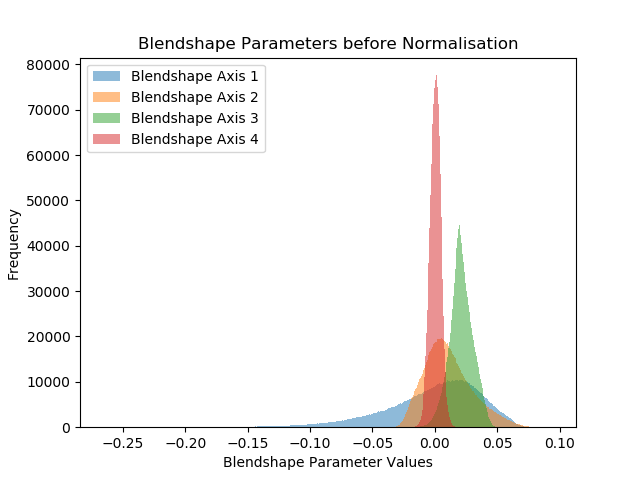
\includegraphics[width=\textwidth]{figures/dataset/shape_params_unnormalised_hist.png}
        \caption{Unnormalised}\label{fig:hist_unnorm}
    \end{subfigure}
    \begin{subfigure}[b]{0.49\textwidth}
        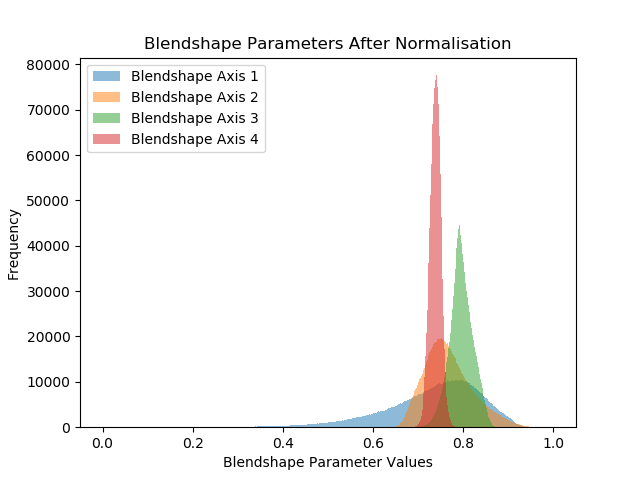
\includegraphics[width=\textwidth]{figures/dataset/shape_params_normalised_hist.png}
        \caption{Normalised}\label{fig:hist_norm}
    \end{subfigure}
    \caption{Blendshape Parameter Histograms}
\end{figure}

\section{Assessment of Model Performance}
In order to assess the performance of the models in the task of word level classification, several metrics exist which could be used.
The chosen metrics are the model accuracy and the Levenshtein Distance.
The accuracy gives a measure of how frequently the model correctly predicts the word while the Levenshtein Distance represents how far the incorrect predictions are from the correct words.

\subsection{Accuracy}
The accuracy of a model is the ratio between the number of predicted labels made by the model which are correct and the total number of predictions.
Accuracy is an appropriate metric in the instance when the dataset is balanced, that is to say that there are an equal number of all labels in the dataset.

If the dataset is unbalanced, the accuracy of a model is less informative.
For example, in the scenario where there is a dataset with two labels \textit{A} and \textit{B} with the data being unbalanced such that label \textit{A} occurs 9 times for frequently than label \textit{B}.
A model which achieves 90\% accuracy on this dataset may be correctly labelling all data 90\% of the time, or it may be labelling all data samples as label \textit{A} without learning anything about the dataset and achieving the same accuracy.

For unbalanced data the F1-Score metric is more useful as this will remain low when a single label class is frequently being incorrectly predicted.
However, as the dataset this problem is concerned with is balanced, this shall not be discussed.

\subsection{Levenshtein Distance}
The Levenshtein Distance is a character level distance between two words defined as the minimum number of single character edits required to make the two the same \cite{Levenshtein1966}.
Single character edits are described as removing a character, substituting for another character and adding a new character.
In the example shown in Figure \ref{fig:levenshtein}
This was used by Chung et al. in \cite{Cheng2016}, although it was defined as the character-level edit distance (section \ref{sec:lip_reading_models}).
This can be calculated for each model prediction and the average character-level edit distance can be found for the model as a whole, or per label.

\begin{figure}[h!]
\centering
    \begin{tabular}{c c c c c l }
        \multicolumn{1}{ c }{} & \\
        A & B & U & S & E & \\
        A & B & O & U & T & \\
        \cline{1-5}
        & & & & & \multicolumn{1}{l}{\textbf{Operation}} \\
        \cline{1-5}
        A & B & U & T & - & Remove O \\
        \cline{1-5}
        A & B & U & S & - & Substitute T for S\\
        \cline{1-5}
        A & B & U & S & E & Add E\\
        \cline{1-5}
    \end{tabular} 
    \caption{Levenshtein Distance Example}
\end{figure}\label{fig:levenshtein}

\section{Model Architecture}

\subsection{Multiple Towers Classification Model}
The first model is based on the Multiple Towers architecture used in \cite{Chung2016} used for lip reading on 2D temporal data with the LRW dataset described in Section \ref{sec:lip_reading_models}.
This is a CNN architecture which firstly applies a convolutional layer to the input image frames separately before concatenating the output feature maps and proceeding to convolve over the time domain.
The original Multiple Towers architecture can be seen in Figure \ref{fig:LRW_Multiple_Towers} while the architecture adapted from this design for prediction from blendshape parameters is shown in Figure \ref{fig:Blendshape_Multiple_Towers}

\subsubsection{Model Input}
The model inputs are in the form of blendshape parameter values for each frame in the motion sequence.
These represent the interpolation from the template mesh as described in section \ref{sec:blendshape_recovery} for each time frame.
For a duration of one second there are 43 frames, 4 blendshape parameters per frame and a single channel dimension, such that the input to the model is $\mat{x} \in \mathbb{R}^{1 \times 4 \times 43}$

\subsubsection{Loss Function}
The model is trained with the Negative Log Likelihood (NLL) on 500 class labels for each of the labels in the dataset.
The model makes word level predictions with the LogSoftmax activation function applied to the final layer of the model.

\subsubsection{Model Architecture}
Similar to the architecture proposed by Chung et al. \cite{Chung2016}, the first convolutional layers do not convolve over the time domain by using 3x1 kernels which do not have a receptive field across the time domain.
These two layers reduce the input shape from $[1 \times 4 \times 43]$ to $[512 \times 1 \times 43]$, encoding the 4 blendshape parameters into a single value across multiple channels, allowing the single dimension to be collapsed and 1D convolutional layers to be used for subsequent layers.

The Multiple Towers architecture used by Chung et al. featured max pooling layers to reduce the size of feature maps.
As a linear layer is to be used at the final layer of the model to facilitate label prediction with a LogSoftmax activation function, it is desirable to reduce the size of the feature maps to prevent the linear layer having too many parameters as this becomes difficult to train and can lead to overfitting.
Max pooling layers reduce the size of feature maps in the network, only retaining the information which is of the most use to the model.

In order to aid in the training of the model, batch normalisation is applied after convolutional layers in all cases except for the final convolutional layer.
Similarly, dropout was applied to all but the final convolution layer in order to assist the model from overfitting the training data.
During training, the model suffered from significant overfitting to the training data, dropout was applied and assist in the prevention of this.
In addition to dropout, weight decay was also used to improve performance on the validation data.
Early stopping was used to prevent the model learning to overfit further on the training data.
This was achieved by keeping a running average of the loss on validation data of the previous 10 epochs, training was stopped once the validation loss stopped decreasing (see Figure \ref{fig:blendshape_multi_tower_loss}).

A detailed breakdown of the model specification can be seen in Table \ref{table:multi_towers_classifier}.
The hyperparameters which provided the optimum results on the validation data are shown in Table \ref{table:multi_towers_classifier_hyperparameters} 

\begin{figure}[h!]
    \centering
        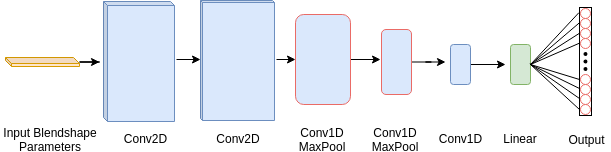
\includegraphics[width=0.9\textwidth]{figures/classification/blendshape_multi_tower_arch.png}
    \caption{Multiple Towers Classification Architecture}
\end{figure}\label{fig:Blendshape_Multiple_Towers}
\quad

\begin{table}[h!]
\centering
    \begin{tabular}{ | l | r | r | r | l | r | l |}
    \hline
    \textbf{Layer} & \textbf{Output} & \textbf{Kernel} & \textbf{Stride} & \textbf{Batch Norm} & \textbf{Dropout} & \textbf{Activation} \\ \hline
    Conv2D & 512x2x43 & 3x1 & 1x1 & True & 0.2 & ReLU \\ \hline
    Conv2D & 512x1x43 & 3x1 & 1x1 & True & 0.2 & ReLU \\ \hline
    Conv1D & 256x41 & 3 & 1 & True & 0.2 & ReLU \\ \hline
    MaxPool & 128x20 & 3 & 2 & - & - & - \\ \hline
    Conv1D & 64x18 & 3 & 1 & True & 0.2 & ReLU \\ \hline
    MaxPool & 64x9 & 3 & 2 & - & - & - \\ \hline
    Conv1D & 64x7 & 3 & 1 & False & 0.0 & ReLU \\ \hline
    Linear & 500 & - & - & False & 0.0 & LogSoftmax \\
    \hline
    \end{tabular} 
    \caption{Multiple Towers Model Architecture}
\end{table}\label{table:multi_towers_classifier}
\quad

\begin{table}[h!]
\centering
    \begin{tabular}{ | l | r | r | r |}
    \hline
    \textbf{Optimisation Algorithm} & \textbf{Learning Rate} & \textbf{Weight Decay} & \textbf{Batch Size} \\ \hline
    RMSprop & 0.0002 & 0.001 & 128 \\
    \hline
    \end{tabular} 
    \caption{Multiple Towers Model Hyperparameters}
\end{table}\label{table:multi_towers_classifier_hyperparameters}


\subsection{Blendshape Channels Classification Model}
The second model applied to this task is not directly inspired by any existing model architecture.
Unlike the Multiple Towers Model, this model convolves over the time domain throughout the whole depth of the model and treats each blendshape axis as a separate channel to the input of the model, thus the model shall be referred to as the Blendshape Channels Model.
As with the previous classification model, NLL is used as a loss function.

\subsubsection{Model Input}
The model inputs, as before are in the form of blendshape parameters values corresponding to frames in the motion sequence.
Unlike the previous model, each blendshape axis is treated as a separate input channel, such that the input data is in the form $\mat{x} \in \mathbb{R}^{4 \times 43}$.
Treating the blendshape axes as separate channels allows the model to extract information from them separately while considering the time domain for each.

TODO, some of this may need to be moved to discussion section.

\subsubsection{Model Architecture}
The Blendshape Channel model is a CNN architecture convolving over the time domain of the input data throughout the whole depth of the model.
Reducing the length of the feature maps as the model deepens, while increasing the number of channels in the feature maps to allow for more fine details to be extracted from the data.

In order to reduce the length of the feature maps in the model, max pooling layers are applied after the 3\textsuperscript{rd} and 5\textsuperscript{th} convolutional layers.
As with the Multiple Towers Model, this forces the model to discard information which is of less importance, while reducing the size of the feature maps.

The final convolutional layer reduces the number of channels in the output feature map in order to reduce the number of parameters in the output linear layer for word level predictions with the LogSoftmax activation function.
Full model specification are shown in Table \ref{table:blendshape_channels_classifier}.
Similar to the Multiple Towers Model, batch normalisation is applied to aid in stabilising the training of the model, while dropout did not improved the performance on the validation data.
The model was tuned on the validation data to with the hyperparameters shown in Table \ref{table:blendshape_channels_classifier_hyperparameters}.

\begin{figure}[h!]
    \centering
        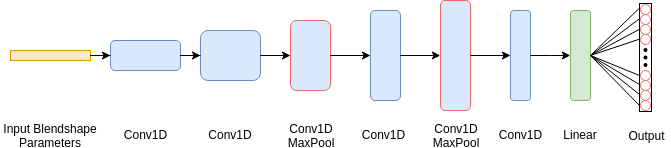
\includegraphics[width=0.9\textwidth]{figures/classification/blendshape_channel_arch.png}
    \caption{Blendshape Channels Classification Architecture}
\end{figure} \label{fig:Blendshape_Channel_Classifier}
\quad

\begin{table}[h!]
\centering
    \begin{tabular}{ | l | r | r | r | l | r | l |}
    \hline
    \textbf{Layer} & \textbf{Output} & \textbf{Kernel} & \textbf{Stride} & \textbf{Batch Norm} & \textbf{Dropout} & \textbf{Activation} \\ \hline
    Conv1D & 4x43 & 3 & 1 & True & 0.0 & ReLU \\ \hline
    Conv1D & 32x41 & 3 & 1 & True & 0.0 & ReLU \\ \hline
    Conv1D & 64x39 & 3 & 1 & True & 0.0 & ReLU \\ \hline
    MaxPool & 128x18 & 3 & 2 & - & - & - \\ \hline
    Conv1D & 256x16 & 3 & 1 & True & 0.0 & ReLU \\ \hline
    Conv1D & 512x14 & 3 & 1 & True & 0.0 & ReLU \\ \hline
    MaxPool & 512x7 & 2 & 2 & - & - & - \\ \hline
    Conv1D & 256x5 & 3 & 1 & False & 0.0 & ReLU \\ \hline
    Linear & 500 & - & - & False & 0.0 & LogSoftmax \\
    \hline
    \end{tabular} 
    \caption{Blendshape Channels Model Architecture}
\end{table}\label{table:blendshape_channels_classifier}
\quad

\begin{table}[h!]
\centering
    \begin{tabular}{ | l | r | r | r |}
    \hline
    \textbf{Optimisation Algorithm} & \textbf{Learning Rate} & \textbf{Weight Decay} & \textbf{Batch Size} \\ \hline
    RMSprop & 0.00005 & 0.005 & 128 \\
    \hline
    \end{tabular} 
    \caption{Blendshape Channels Model Hyperparameters}
\end{table}\label{table:blendshape_channels_classifier_hyperparameters}

\section{Results}

\subsection{Multiple Towers Model}

\begin{figure}[h!]
    \centering
    \begin{subfigure}[b]{0.49\textwidth}
        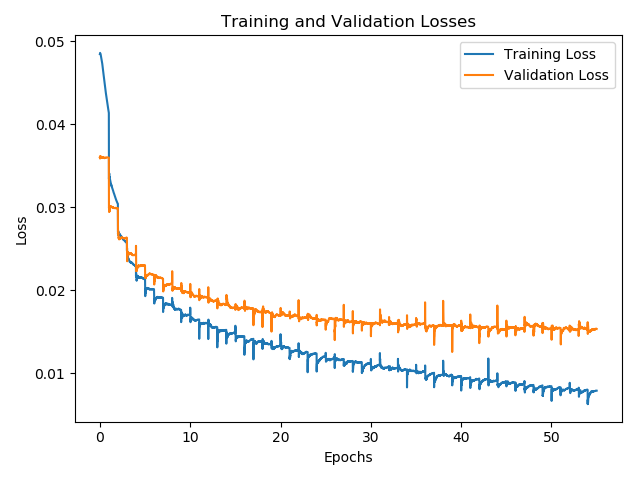
\includegraphics[width=\textwidth]{figures/classification/blendshape_multi_tower_loss.png}
        \caption{Losses}\label{fig:blendshape_multi_tower_loss}
    \end{subfigure}
    \begin{subfigure}[b]{0.49\textwidth}
        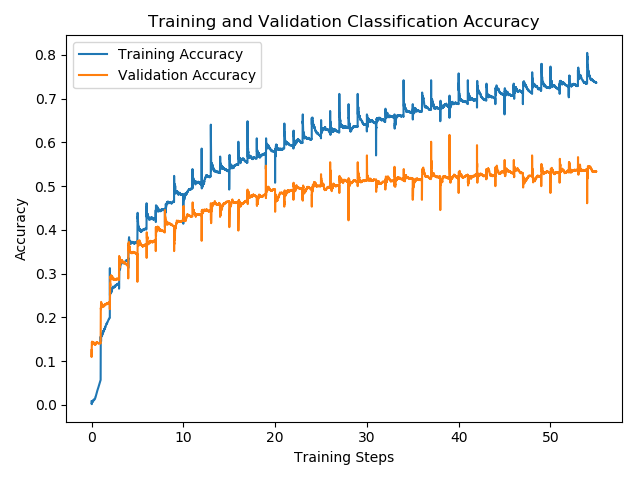
\includegraphics[width=\textwidth]{figures/classification/blendshape_multi_tower_acc.png}
        \caption{Accuracy}\label{fig:blendshape_multi_tower_acc}
    \end{subfigure}
    \caption{Multiple Towers Training}\label{fig:multiple_towers_training}
\end{figure}

\begin{figure}[h!]
    \centering
        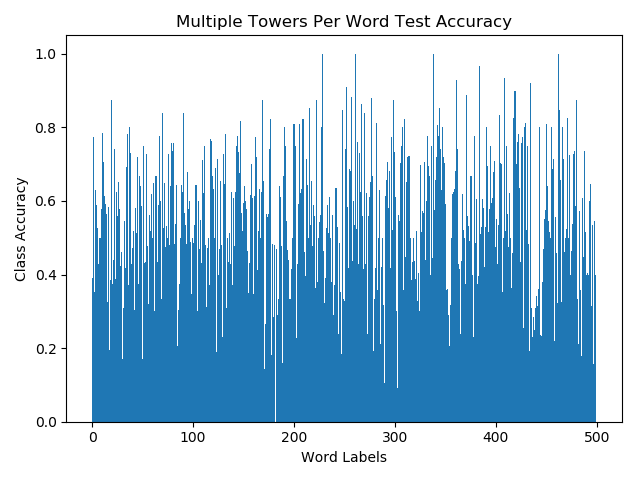
\includegraphics[width=0.7\textwidth]{figures/classification/blendshape_multi_tower_class_acc.png}
    \caption{Blendshape Multi Tower Class Accuracy}
\end{figure} \label{fig:Blendshape_Multi_Tower_Class_Acc}

\begin{figure}[h!]
    \centering
    \begin{subfigure}[b]{0.49\textwidth}
        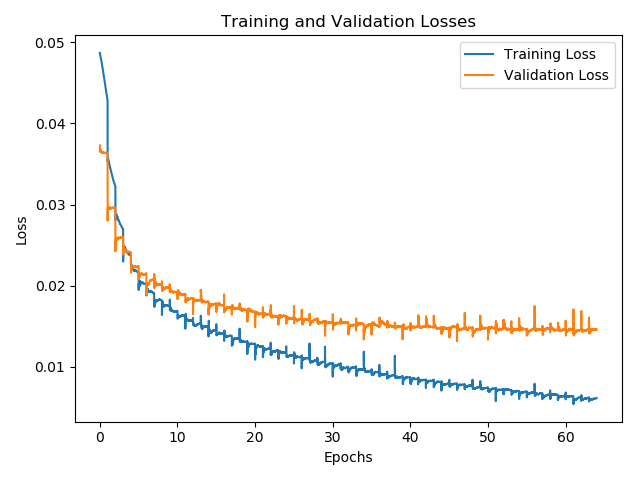
\includegraphics[width=\textwidth]{figures/classification/blendshape_channel_loss.png}
        \caption{Losses}\label{fig:blendshape_channel_loss}
    \end{subfigure}
    \begin{subfigure}[b]{0.49\textwidth}
        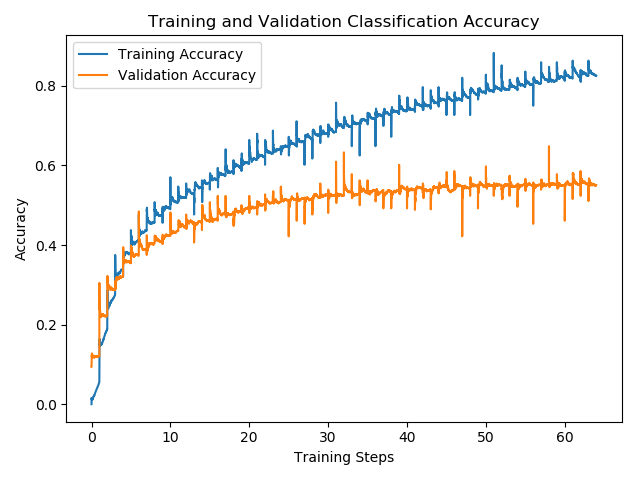
\includegraphics[width=\textwidth]{figures/classification/blendshape_channel_acc.png}
        \caption{Accuracy}\label{fig:blendshape_channel_acc}
    \end{subfigure}
    \caption{Blendshape Channels Training}
\end{figure}

\begin{figure}[h!]
    \centering
        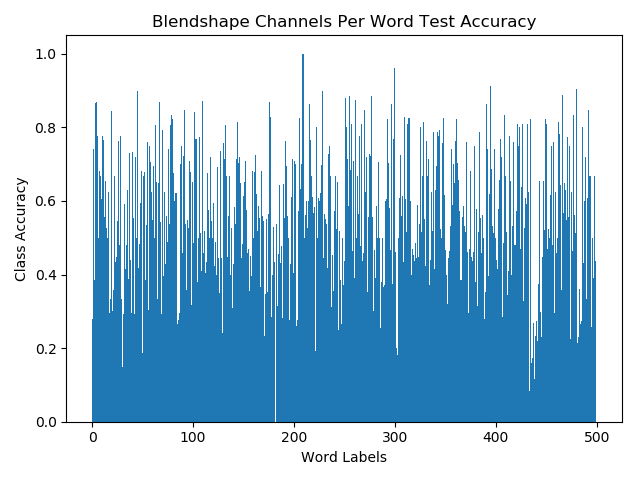
\includegraphics[width=0.7\textwidth]{figures/classification/blendshape_channel_class_acc.png}
    \caption{Blendshape Channels Class Accuracy}
\end{figure} \label{fig:Blendshape_Channels_Class_Acc}

\begin{figure}[h!]
    \centering
    \begin{subfigure}[b]{0.49\textwidth}
        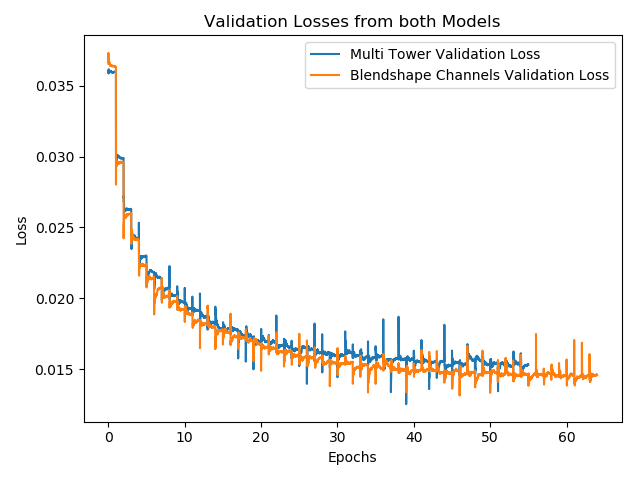
\includegraphics[width=\textwidth]{figures/classification/both_models_val_loss.png}
        \caption{Losses}\label{fig:both_models_val_loss}
    \end{subfigure}
    \begin{subfigure}[b]{0.49\textwidth}
        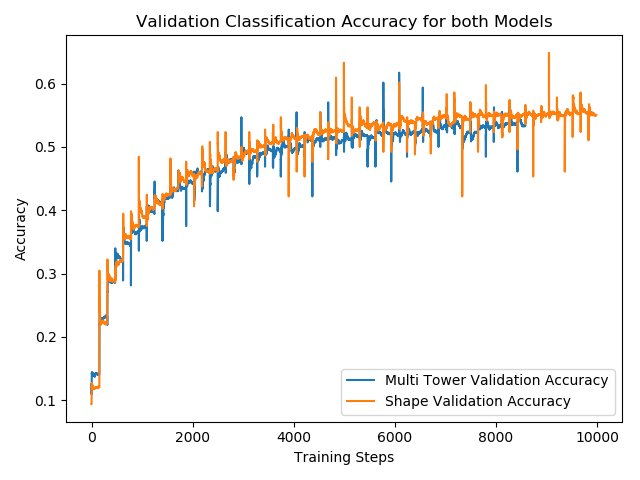
\includegraphics[width=\textwidth]{figures/classification/both_models_val_acc.png}
        \caption{Accuracy}\label{fig:both_models_val_acc}
    \end{subfigure}
    \caption{Model Training Comparison}
\end{figure}

\section{Discussion}

%\bibliographystyle{unsrt}
%\bibliography{ref}
%\end{document}


%%%%%%%%%%%%%%%%%%%%%%%%%%%%%%%%%%%%
\externaldocument{clendshape_classification}
\externaldocument{lit_review}

\chapter{Audio Driven Blendshape GAN}
This chapter shall discuss the use of GANs for audio driven facial animation.
Unlike previous generative models which solve a regression problem to correctly match an audio input to a sequence parameters which describe facial motion, GANs also include an noise input resulting in variations in the output from the same conditional input.
The model outputs will then be assessed on the classification models discussed in Chapter \ref{chap:classification}.
The GAN is comprised of two neural networks, a Generator and a Critic, which are trained together using the outputs of each network to train the other.

\section{Problem Definition}
Currently, there is a lack of 3D temporal datasets which sync speech audio with corresponding facial motion with the purpose of training a model for VSR.
Such datasets are difficult to capture directly due to the equipment and time required.
Similar datasets exist which have enabled for the creation of audio driven models but these datasets are limited in size and variation and have led to models which are specific to subjects either though direct subject specific training data as with the model by Karras et al. \cite{Karras2017a} or through character encoding, as is the case with the VOCA model \cite{Cudeiro2019}.
Through the use of these models, a synthetic dataset of 3D temporal facial motion was generated as described in Section \ref{sec:dataset_gen}.
This data however is subject to all biases and restrictions the VOCA model is subject to.
An appropriate dataset would contain a small vocabulary, similar to the LRW dataset of 500 words, all spoken by multiple subjects to capture different speaking styles for the same words captured from `\textit{in the wild}' scenarios.

An appropriate dataset would:
\begin{itemize}
    \item A small vocabulary of a similar size to the LRW dataset.
    \item Multiple subjects speaking the same vocabulary to capture different speaking styles for the same words.
    \item ``\textit{In the wild}'' audio conditions.
\end{itemize}

As a means to increase the variation in speaking style in existing audio drive generative models such as VOCA, a GAN model is to be trained on the data generated by the VOCA model and the original LRW audio from which the VOCA generated dataset was driven from.
The resulting generative model should be able to replicate the results of the VOCA model, but with increased variation in speaking styles due to the noise input component.

\section{Model Inputs}
The generative model is to be driven from an audio input of audio samples from the LRW dataset which were used as inputs to the VOCA model to generate the dataset of blendshape parameters.
Audio data in the time domain has a high number of samples per second to allow all frequencies observable by human hearing to be captured.
Human hearing can commonly hear up to 20kHz, which results in a sample rate of at least 40kHz to meet the Nyquist sampling rate, which states that the sample rate must be at least twice the desired maximum observable frequency to accurately represent the signal at this frequency.
40,000 samples for a single second is however, is a large number of samples and an inefficient data representation.
Commonly audio data is converted to the frequency domain which allows for a far more efficient means of data representation. 

\subsection{Mel-frequency Cepstral Coefficients}
Common implementations of machine learning models which use audio as in input, focused on speech, have used Mel-frequency cepstral coefficients (MFCCs) to represent audio.
\textcolor{red}{TODO add references to paper examples.}
MFCCs were inspired by human anatomy and speech, invented by Davis and Mermelstein in 1980 \cite{Davis1980}.
Human speech is naturally filtered by the shape of the shape of the mouth and vocal tract.
This envelope can be well represented by the short time power spectrum.
A large amount of information is contained within an audio sample in the time domain, much of which does not contain meaningful information.
By filtering the audio sample in the frequency domain to this envelope, information useful to speech detection is maintained while other information is discarded.

Firstly the assumption that over a short time frame, the audio signal does not statistically vary greatly.
This assumption allows the signal to be split into short frames which can be processed separately.
An example of the audio frames is show in Figure \ref{fig:mfcc_audio_frames}.

\begin{figure}[h!]
    \centering
        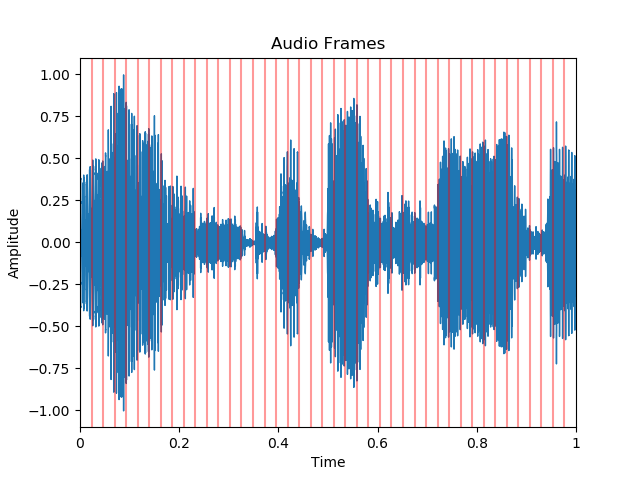
\includegraphics[width=0.7\textwidth]{figures/mfcc/audio_frames.png}
    \caption{Audio Sample Frames}\label{fig:mfcc_audio_frames}
\end{figure} 

For each frame the power spectrum is calculated using the periodogram estimation.  
The incentive behind calculating the power spectrum is derived from human anatomy, specifically from the cochlea.
The cochlea is a bone which resides within the ear and different parts of the bone vibrate depending on the frequency of the incoming audio signal.
The periodogram estimation of the power spectrum performs a similar operation by identifying which frequencies are present within an audio signal.
This representation still retains information which is not useful for speech recognition, for example the cochlea cannot distinguish between closely spaced frequency values, this is more apparent at higher frequencies.
The power spectrum for a single audio frame is shown in Figure \ref{fig:mfcc_power_spec}.
For this reason a series of Mel filterbanks are applied to the power spectrum and the resulting bin for each filter is summed, this gives an approximation of the energy present in each frequency region.
The Mel filterbanks are visualised in Figure \ref{fig:mfcc_mel_filterbanks}.
The log of each summation is then taken as humans do not perceive loudness on a linear scale, so the log compression matches the features more closely to what humans hear, shown in Figure \ref{fig:mfcc_log_sum}.

\begin{figure}[h!]
    \centering
    \begin{subfigure}[b]{0.49\textwidth}
        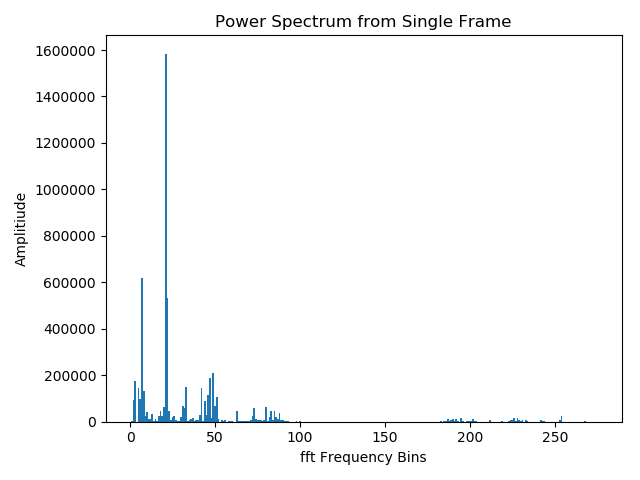
\includegraphics[width=\textwidth]{figures/mfcc/frame_power_spectrum.png}
        \caption{Audio Frame Power Spectrum}\label{fig:mfcc_power_spec}
    \end{subfigure}
    \begin{subfigure}[b]{0.49\textwidth}
        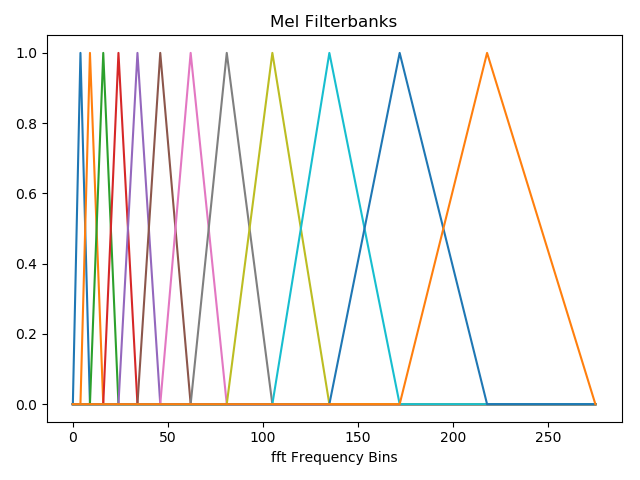
\includegraphics[width=\textwidth]{figures/mfcc/filterbanks.png}
        \caption{Mel Filterbanks}\label{fig:mfcc_mel_filterbanks}
    \end{subfigure}
    \caption{Mel Filterbank Processing}\label{fig:mfcc_filterbank_processing}
\end{figure}

Lastly, the Discrete Cosine Transformation is applied to the each filterbank energy, this is performed to decorrelate the filterbanks are they are highly correlated due to the overlap in the Mel filters, the resulting representation is shown in Figure \ref{fig:mfcc_dct}.
This represents the MFCC values for a single audio frame for 8 Mel filterbanks.

\begin{figure}[h!]
    \centering
    \begin{subfigure}[b]{0.49\textwidth}
        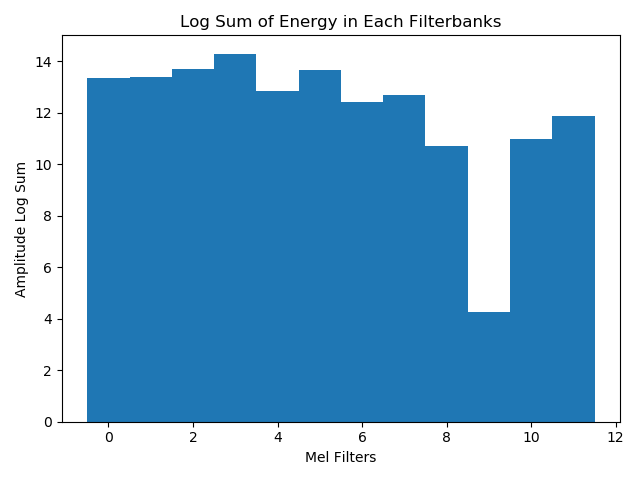
\includegraphics[width=\textwidth]{figures/mfcc/filterbank_log_sum.png}
        \caption{Log Sum}\label{fig:mfcc_log_sum}
    \end{subfigure}
    \begin{subfigure}[b]{0.49\textwidth}
        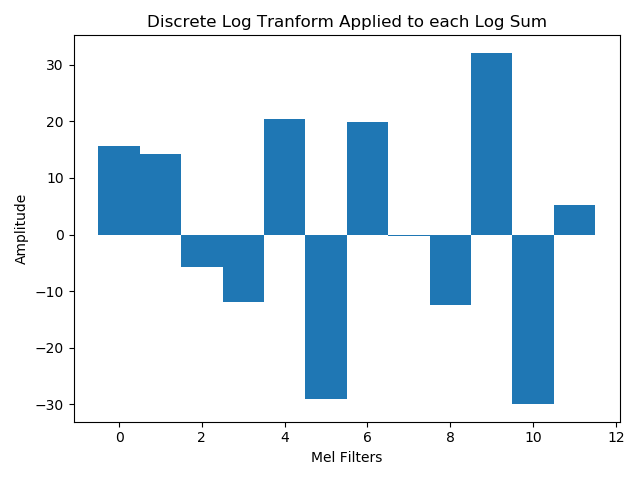
\includegraphics[width=\textwidth]{figures/mfcc/dct_applied.png}
        \caption{Discrete Cosine Transformation}\label{fig:mfcc_dct}
    \end{subfigure}
    \caption{Discrete Cosine Transformation Processing}\label{fig:mfcc_filterbank_processing}
\end{figure}

The model inputs use a total of 12 filterbanks over the span of one second audio clips.
This results in an model input MFCC $\mat{x} \in \mathbb{R}^{12 \times 43}$, visualised in Figure \ref{fig:mfcc_model_input}.

\begin{figure}[h!]
    \centering
    \begin{subfigure}[b]{0.49\textwidth}
        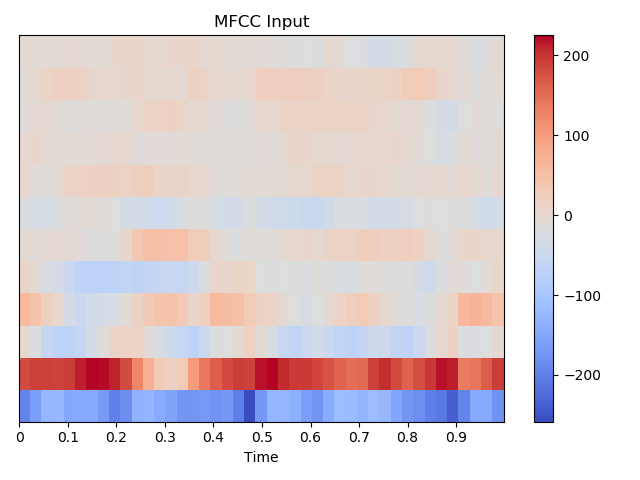
\includegraphics[width=\textwidth]{figures/mfcc/mfcc_input.png}
        \caption{MFCC Model Input}\label{fig:mfcc_input}
    \end{subfigure}
    \begin{subfigure}[b]{0.49\textwidth}
        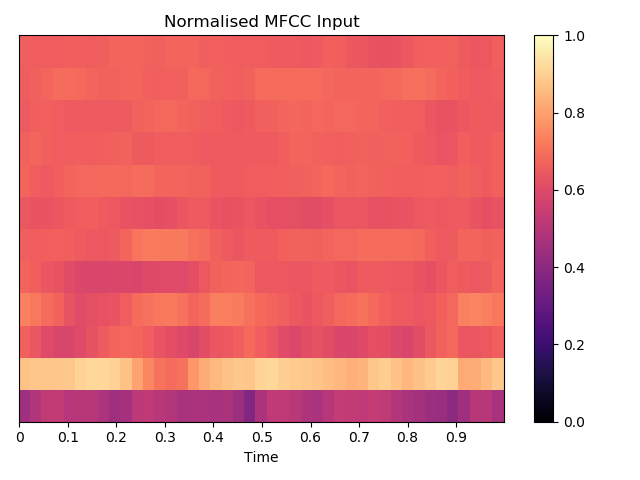
\includegraphics[width=\textwidth]{figures/mfcc/norm_mfcc_input.png}
        \caption{Normalised MFCC Model Input}\label{fig:mfcc_norm_input}
    \end{subfigure}
    \caption{MFCC Model Input}\label{fig:mfcc_model_input}
\end{figure}

\subsection{Blendshape Inputs}
The Generator aims to produce realistic blendshape parameters for the input audio signal, thus the input to the Critic must be the true blendshape parameter values and the `fake' generated blendshape parameters.
These values are the same as were input to the Blendshape Classification models discussed in Section \ref{sec:classification_inputs}: $\mat{y} \in \mathbb{R}^{4 \times 43}$.
The reader is directed to this section for further details.

\subsection{Noise Input}
In addition to audio represented in the form of MFCCs, the Generator is also input with a noise component consisting of random samples taken from a uniform probability distribution within the range of 0 and 1, expressed by equation (\ref{eq:uniform_dist}).

\begin{equation}\label{eq:uniform_dist}
    f(x)=\begin{cases}
      \frac{1}{b-a}, & \text{for $a \leq x \leq b$}\\
      0, & \text{elsewhere}
    \end{cases}
\end{equation}

\section{Data Preprocessing}
As with the classification models, data inputs to the model are normalised within the range [0,1], the normalised MFCC input is shown in Figure \ref{fig:mfcc_norm_input}.
This normalisation makes training both the critic and the generator easier as the range of values which the model will observe is reduced while preserving the statistical properties of the data.
As the generated blendshape parameters are within the range [0,1] the Sigmoid activation function can be used at the output layer of the model, rather than a linear output with an infinite range.

\section{Assessment of Model Performance}
Assessing the performance of GAN is less straightforward than other machine learning models.
For example, in a supervised learning scenario, a classification model can be assessed on the accuracy of predictions or f-score on a test set in addition to the model loss on these predictions, as discussed in Section \ref{sec:class_assessment}.
As GAN describe an unsupervised learning scenario, assessment metrics are less clear and problem specific.
In this problem, the aim of the Generator is to find a mapping from an audio signal represented by a series of MFCCs, to a series of blendshape parameters which the Critic considers to be a correct match.
The Critic's goal is to be able to judge pairings of MFCCs and blendshape parameters as a realistic match.

A realistic pairing of audio and blendshape parameters would meet the following conditions:
\begin{itemize}
    \item Movement would appear realistic to a human observer.
    \item Movement would appear correlated to the speech in the audio signal to a human observer.
    \item Speech would be correlated, such that a pretrained blendshape classifier would be able to make some degree of successful predictions from the parameters.
\end{itemize}

The first two conditions are difficult to evaluate in a quantitative manner as this is a matter of opinion from the observer.
A subjective evaluation can be conducted on a collection of participants, however finding subjects who can accurately lip read is challenging due to the difficulty of the skill, especially in this scenario where there is no context for the spoken phrases.
Subjects who cannot lip read could be used, however this is unreliable as in many cases a video clip which has been dubbed over with an audio signal, which has been roughly matched with a speaking subject may seem plausible.
With the absence of audio, the 'realism' of the animation movement is also difficult to determine.
While aspects of animation which easily make generated data identifiable are sudden movements and shaking in the animation which would not be apparent in real speech, a series of parameter values which produce a smooth animation may easily fool observers.

A quantitative metric which can be evaluated is the performance of generated samples on the pretrained blendshape classifiers, the architecture and performance of which is discussed in Chapter \ref{chap:classification}.
As the Generator aims to find the mapping between the input audio signal and blendshape parameters, if successful, the generated blendshape parameters should have properties similar to those of the original data which would allow for correct classification.

Given that the success of the Generator is dependent upon producing blendshape parameters which the critic cannot distinguish from real samples, the primary metric which shall be used is the losses on the validation set from both the Critic and the Generator during training.
Training of the Generator will be complete when the Critic can no longer distinguish between real and fake samples.
Will this occurs the Critic losses have settled at 0.

\section{Model Architecture}
The GAN is composed of a Generator and a Critic, trained with the Wasserstein Loss with Gradient Penalty to ensure the Lipschtiz condition, described by equation (\ref{eq:wgan_gp}).
More details on the loss function is discussed are Section \ref{sec:Stability_to_GANs}.

\subsection{Model Structure}
The GAN model is trained with Wasserstein Loss with Gradient Penalty to meet Lipschtiz condition as discussed in Section \ref{sec:Stability_to_GANs}.
The GAN model is constructed of two CNN architectures; a Generator and a Critic.
A high level diagram of the GAN model is shown by Figure \ref{fig:gan_model}.

\begin{figure}[h!]
    \centering
        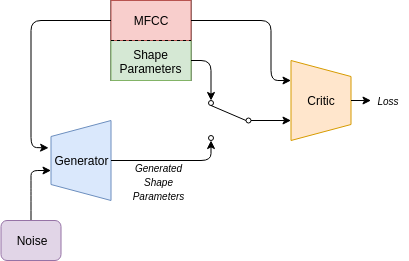
\includegraphics[width=0.9\textwidth]{figures/gan/gan.png}
    \caption{GAN Model}\label{fig:gan_model}
\end{figure} 

The Critic is trained on a corresponding pair of MFCC values and blendshape parameters.
The goal of the Critic is to be able to identify a correct pairing from the dataset and a false pairing consisting of MFCC values and a fake series of blendshape parameters generated by the Generator.
The Critic returns a score value within the range of [-1, 1], where data inputs which it regards as realistic are smaller, while parings which is regards as fake are larger.
For each minibatch in a training epoch the Critic is shown a batch of real data values $\mat{x}$ and the Generator creates a batch of fake data values $\mat{\tilde{x}}$.
The Critic evaluates this data and returns a score for both the real and fake data.
In addition to the loss from the Critic score on real and fake data samples, the gradient penalty term is calculated, this term is to be minimised to meet the Lipschtiz condition, \cite{Gulrajani2017}.
This is found by evaluating the score of the Critic on a new data sample taken at random along the interpolation between the real and fake blendshape parameters, $\mat{\hat{x}}$.
The gradient penalty term $\mat{k}$ can then be found with equation (\ref{eq:grad_penalty}) with the interpolated value, where $\lambda$ is a tunable hyperparameter.

\begin{equation}\label{eq:grad_penalty}
    \mat{k} = \lambda \E{\bm{\hat{x}} \sim \Pd{\bm{\hat{x}}}} 
            [(\| \nabla_{\bm{\hat{x}}} D(\bm{\hat{x}}) \| - 1)^2]
\end{equation}

The Generator takes inputs of MFCC values and noise from a uniform distribution, these are concatenated together and processed as a single input.
The Generator then attempts to map this input into blendshape parameter values which the Critic evaluated to a low loss value. 
During training, the samples produced by the Generator are assessed by the Critic.
The Generator aims to have the samples it produces labelled as realistic, such that the Critic returns a low value.

At any point for the Generator to improve the quality of the samples it can produce, the Critic must initially be able to distinguish between the real and fake samples, else the Generator has no incentive to improve.
For this reason, the Critic is trained more frequently then the Generator, in this case the Generator is trained one in ten batches, while the Critic is trained on every batch, the data is shuffled so that the Generator is still exposed to the whole training dataset.

\begin{table}[h!]
\centering
    \begin{tabular}{l | r | r}
    & \textbf{Generator} & \textbf{Critic}\\
    \hline
    Optimisation Algorithm & RMSprop & RMSprop \\
    Learning Rate          & 0.00001 & 0.00001 \\
    Scheduler              & 0.999   & 0.999   \\
    Batch Size             & 128     & 128     \\
    Training Ratio         & 1:10    & 1:1     \\
    Gradient Penalty       & -       & 5       \\
    \end{tabular} 
    \caption{GAN Hyperparameters}\label{table:gan_hyperparameters}
\end{table}

\subsection{Generator}
The Generator aims to transform noise from a uniform distribution into realistic blendshape parameters given the conditional input of MFCC values for a given audio sample.
Five channels of noise are sampled with the same shape as in MFCC input and the two are concatenated along the channel dimension, such that the input data is $\mat{z} \in \mathbb{R}^{6 \times 12 \times 43}$.
The Generator model architecture is a fully convolutional network which takes the input values $\mat{z}$ and transforms this into blendshape parameters $\mat{\tilde{x}} \in \mathbb{R}^{4 \times 43}$.

\begin{figure}[h!]
    \centering
        \includegraphics[width=0.8\textwidth]{figures/gan/generator.png}
    \caption{Generator Model Architecture}\label{fig:gan_gen_arch}
\end{figure}

The model (shown in Figure \ref{fig:gan_gen_arch}) consists of five convolutional layers, the detailed specification of which is shown in Table \ref{table:gan_gen_arch}.
The first pads the input along the time domain as the output dimension along the time domain is to be the same as in input, corresponding to separate frames of blendshape parameters, without padding this dimension would be reduced due to convolution operations.
This is a significant amount of padding to be applied to a single layer, however when a padding values of one was applied to all layers this resulted obvious artifacts at the beginning and end of the generated sequence, while this produces no such artifacts.
The first layer has a high number of filter channels to extract the largest possible amount of information from in input data, following layers reduce the number of channels to compress this information into the final output layer which has 4 channels, one for each blendshape parameter.

The model uses ReLU activate functions for all hidden layers and the Sigmoid activation function at the output layer to achieve blendshape parameters in the range [0, 1].
The output layer also uses a larger kernel size than the hidden layers, which all use a kernel size of 3.
When a small kernel was used at the output layer there existed a large amount of of jitter in the output parameters, increasing the output kernel seems to eliminate this and produce animation with smoother motion.
The role of this output layer is not to extract useful information for subsequent layers to use, but to generate the output values.
A larger kernel increases to receptive field of this layer on the feature maps from the previous layer, resulting in reduced variation between subsequent frames and less jitter.

\begin{table}[h!]
\centering
    \begin{tabular}{ l | r | r | r | l}
    \textbf{Layer} & \textbf{Output} & \textbf{Kernel} & \textbf{Padding} & \textbf{Activation} \\ \hline
    Conv2D & 256x10x53 & (3,3) & (0,6) & ReLU    \\ \hline
    Conv2D & 128x8x51  & (3,3) & (0,0) & ReLU    \\ \hline
    Conv2D & 128x6x49  & (3,3) & (0,0) & ReLU    \\ \hline
    Conv2D & 64x4x47   & (3,3) & (0,0) & ReLU    \\ \hline
    Conv2D & 4x1x43    & (4,5) & (0,0) & Sigmoid 
    \end{tabular} 
    \caption{Generator Model Architecture}\label{table:gan_gen_arch}
\end{table}

\subsection{Critic}
The Critic aims to distinguish real data samples from the training dataset from data samples from the Generator.
The high level overview of the model architecture is shown in Figure \ref{fig:gan_critic_arch} and listed in detail in Table \ref{table:gan_critic_arch}.
Inputs to the Critic are comprised of MFCC values and blendshape parameters, both of which have different dimension sizes, but share a common time dimension. 
There are 12 MFCC filter values and 4 blendshape parameter per time instance.
In order to concatenate these values together, the blendshape parameter values are treated as a separate channel and duplicated 12 times, such that the blendshape parameters are expressed as $\mat{b} \in \mathbb{R}^{4 \times 12 \times 43}$.
This is then concatenated with the MFCC values $\mat{m} \in \mathbb{R}^{1 \times 12 \times 43}$, into the input values $\mat{x} \in \mathbb{R}^{5 \times 12 \times 43}$.

The Critic model consists of three sections, the first two are built of convolutional layers using the LeakyReLU activation function while the last the output layer, a linear layer using the Tanh activation function.
the first three layers are two dimensional convolutional layers which do not convolve over the time domain, just the height dimension.
This allows the model to find an efficient encoding of the input audio and blendshape parameters.
The number of filters is increased throughout this encoding stage as opposed to extracting a large number of filters initially as was the case with the Generator.
The reasoning behind this is that the initial input contains a great deal of repetition due to the blendshape parameters being duplicated into the same shape as the MFCC values.

The second section aims to convolve over the time domain, as the singleton dimension can now be collapsed, one dimension convolutional layers can now be used to achieve this.
The section consists of three convolutional layers, each of which have a stride of two and a decreasing kernel size across the three layers.
The first of which uses a kernel size of 5 in order to capture higher level features while the subsequent layers have kernel sizes of 4 and 3 respectively to capture more fine detailed features.

The final layer is a linear layer which provides the critic score for the input data sample.
The layer uses the Tanh activation function to output a score in the range of [-1, 1].

\begin{figure}[h!]
    \centering
        \includegraphics[width=0.9\textwidth]{figures/gan/critic.png}
    \caption{Critic Architecture}\label{fig:gan_critic_arch}
\end{figure}
\quad

\begin{table}[h!]
\centering
    \begin{tabular}{ l | r | r | r | l}
    \textbf{Layer} & \textbf{Output} & \textbf{Kernel} & \textbf{Stride} & \textbf{Activation} \\ \hline
    Conv2D & 64x5x43   & (4,1) & (1,1) & LeakyReLU \\ \hline
    Conv2D & 128x3x43  & (3,1) & (1,1) & LeakyReLU \\ \hline
    Conv2D & 128x1x43  & (3,1) & (1,1) & LeakyReLU \\ \hline
    Conv1D & 128x20    & 5     & 2     & LeakyReLU \\ \hline
    Conv1D & 128x9     & 4     & 2     & LeakyReLU \\ \hline
    Conv1D & 64x4      & 3     & 2     & LeakyReLU \\ \hline
    Linear & 16        & -     & -     & Tanh      
    \end{tabular} 
    \caption{Critic Model Architecture}\label{table:gan_critic_arch}
\end{table}
\quad


\section{Results}

\section{Discussion}


%%%%%%%%%%%%%%%%%%%%%%%%%%%%%%%%%%%%
\chapter{Conclusions and Future Work}

This chapter shall discuss the successes and failures of the project as a whole, both in terms of the successes of the individual models trained and the implications of these findings.
In light of this, the steps which can be taken in future work shall be explored in both the areas of lip reading with blendshape parameters and generative models to produce 3D temporal data for the purpose of lip reading tasks.

\section{Blendshape Classification}\label{sec:class_conc}
This report aimed to investigate as to whether 3D facial data includes information which is of use for word level speech prediction.
To achieve this, firstly a lower dimension representation of a 3D facial mesh was constructed with the use of Principal Component Analysis, referred to as the Blendshape Axes.
Each facial mesh could then be expressed as an interpolation along each Blendshape Axis from a template facial mesh, expressed by the Blendshape Parameters.
This representation of the 3D facial meshes allows for word level prediction for the 500 labels found in the Lip Reading Words Dataset with a mean test accuracy above 50\% for all model architectures investigated.
This demonstrates that firstly, there exists a strong correlation in the facial motion and the words spoken and secondly that this low dimension representation of the data effectively captures this data.

\subsection{Future Work}
The classification models are currently limited to word level prediction of a fixed sequence length and are unable to predict unknown word labels.
A future extension of this work would be to build a model which can perform character level prediction of variable sequence length.
This would allow for the prediction of entire sentences end to end, of variable sequence length.
In order to achieve this, a new dataset would have to be constructed containing sequence frames labelled on a character level.
This could be achieved with the existing dataset used by processing the audio data with a speech recognition system capable of character level prediction per frame, such as the DeepSpeech model.

Secondly, it should be noted that as a large amount of human lip reading relies on the context of the word in the current sentence, incorporating this context, either at a word or character level would likely prove beneficial to model performance.

Given that the classification models have successfully shown that there does exist a correlation between facial motion and speech, a practical application for these findings would be to apply visual speech prediction in a noisy environment where traditional audio speech recognition may perform poorly.
A suggested implementation of this would be to combine predictions from both audio speech recognition and visual speech recognition with the means of a depth camera.
The fusion of these two predictions produces an aggregate model, increasing the likelihood of correct predictions.

\section{Generative Models}
In addition to investigating the use of 3D facial meshes as a means of speech prediction, this report also investigated the use of a Generative Adversarial Network (GAN) to generate Blendshape Parameters driven by an audio input.
The primary incentives behind this were that the current acquisition of 3D temporal data is currently difficult which resulted in the use of existing audio driven facial animation models to be used to construct the dataset on which all models were trained.
This data however is limited in the variations of facial animation for given audio inputs.
With the intention of generating realistic facial animation from an audio input while having a larger variations in facial motion such that classification models may learn to generalise better to unseen data.

The model however proved unsuccessful in achieving this goal.
Generated samples appeared to be correlated with audio samples to human observers, but failed to contain features which are correlated to the words spoken within the audio itself when evaluated with the classification models trained beforehand.
Regardless of the failure of this generative model, generating synthetic data remains an area which should be further pursued while data acquisition of 3D facial scans retains a large barrier to entry.

\subsection{Future Work}
The generative and classification models in this report were trained on data not directly captured due to the difficulties of obtaining such data with the purpose of lip reading.
A primary area of work would be to directly obtain such a dataset, this would allow for a better assessment of the use of GANs as a means of generating synthetic data to augment this with.

The GAN trained in this report was trained with a Critic used to distinguish between real and fake data samples given an audio input and the real or fake generated Blendshape Parameters.
An extension of this would be to train the Generator on both the loss from the Critic and a pretrained classification model.
This may allow for the Generator to learn the features which are present in the data which are correlated to the speech in the audio.
However, this risks the Generator learning to trick the classification model without learning to generalise to unseen audio samples.
Given that the current mean test accuracy of the classification models trained in this report is around 50\%, this may not be an effective means to force the Generator to learn the features which it has currently failed to.

An alternate method of training the GAN would be to drive the generation from a character level conditional input, as opposed to audio driven conditional input.
This would require the model to be able to be trained on variable length input sequence, which in turn would require a dataset labelled on a character level as discussed in Section \ref{sec:class_conc}.
This could be trained either in combination with an audio input on without.



%%%%%%%%%%%%%%%%%%%%%%%%%%%%%%%%%%%%
\chapter*{Ethics}

\begin{longtable}{ p{.80\textwidth} | c | c }
         & Yes & No \\ \hline
        \textbf{Section 1: HUMAN EMBRYOS/FOETUSES} & &  \\ \hline
        Does your project involve Human Embryonic Stem Cells? & & \checkmark \  \\ \hline
        Does your project involve the use of human embryos? & & \checkmark \  \\ \hline
        Does your project involve the use of human foetal tissues / cells? & & \checkmark \  \\ \hline
        \textbf{Section 2: HUMANS} & \  & \  \\ \hline
        Does your project involve human participants? & & \checkmark \  \\ \hline
        \textbf{Section 3: HUMAN CELLS / TISSUES} & \  & \  \\ \hline
        Does your project involve human cells or tissues? (Other than from ``Human Embryos/Foetuses'' i.e. Section 1)? & & \checkmark \  \\ \hline
        \textbf{Section 4: PROTECTION OF PERSONAL DATA} & \  & \  \\ \hline
        Does your project involve personal data collection and/or processing? & & \checkmark \  \\ \hline
        Does it involve the collection and/or processing of sensitive personal data (e.g. health, sexual lifestyle, ethnicity, political opinion, religious or philosophical conviction)? & & \checkmark \  \\ \hline
        Does it involve processing of genetic information? & & \checkmark \  \\ \hline
        Does it involve tracking or observation of participants? It should be noted that this issue is not limited to surveillance or localization data. It also applies to Wan data such as IP address, MACs, cookies etc. & & \checkmark \  \\ \hline
        Does your project involve further processing of previously collected personal data (secondary use)? For example Does your project involve merging existing data sets? & & \checkmark \  \\ \hline
        \textbf{Section 5: ANIMALS} & \  & \  \\ \hline
        Does your project involve animals? & & \checkmark \  \\ \hline
        \textbf{Section 6: DEVELOPING COUNTRIES} & \  & \  \\ \hline
        Does your project involve developing countries? & & \checkmark \  \\ \hline
        If your project involves low and/or lower-middle income countries, are any benefit-sharing actions planned? & & \checkmark \  \\ \hline
        Could the situation in the country put the individuals taking part in the project at risk? & & \checkmark \  \\ \hline
        \textbf{Section 7: ENVIRONMENTAL PROTECTION AND SAFETY} & \  & \  \\ \hline
        Does your project involve the use of elements that may cause harm to the environment, animals or plants? & & \checkmark \  \\ \hline
        Does your project deal with endangered fauna and/or flora /protected areas? & & \checkmark \  \\ \hline
        Does your project involve the use of elements that may cause harm to humans, including project staff? & & \checkmark \  \\ \hline
        Does your project involve other harmful materials or equipment, e.g. high-powered laser systems? & & \checkmark \  \\ \hline
        \textbf{Section 8: DUAL USE} & \  & \  \\ \hline
        Does your project have the potential for military applications? & & \checkmark \  \\ \hline
        Does your project have an exclusive civilian application focus? & & \checkmark \  \\ \hline
        Will your project use or produce goods or information that will require export licenses in accordance with legislation on dual use items? & & \checkmark \  \\ \hline
        Does your project affect current standards in military ethics e.g., global ban on weapons of mass destruction, issues of proportionality, discrimination of combatants and accountability in drone and autonomous robotics developments, incendiary or laser weapons? & & \checkmark \  \\ \hline
        \textbf{Section 9: MISUSE} & \  & \  \\ \hline
        Does your project have the potential for malevolent / criminal / terrorist abuse? & \checkmark & \  \\ \hline
        Does your project involve information on/or the use of biological, chemical, nuclear/radiological-security sensitive materials and explosives, and means of their delivery? & & \checkmark \  \\ \hline
        Does your project involve the development of technologies or the creation of information that could have severe negative impacts on human rights standards (e.g. privacy, stigmatization, discrimination), if misapplied? & & \checkmark \  \\ \hline
        Does your project have the potential for terrorist or criminal abuse e.g. infrastructural vulnerability studies, cybersecurity related project? & & \checkmark \  \\ \hline
        \textbf{SECTION 10: LEGAL ISSUES} & \  & \  \\ \hline
        Will your project use or produce software for which there are copyright licensing implications? & & \checkmark \  \\ \hline
        Will your project use or produce goods or information for which there are data protection, or other legal implications? & & \checkmark \  \\ \hline
        \textbf{SECTION 11: OTHER ETHICS ISSUES} & \  & \  \\ \hline
        Are there any other ethics issues that should be taken into consideration? & & \checkmark \  \\ 
\end{longtable} 

\section*{Ethical Considerations of this Report}

    


%%%%%%%%%%%%%%%%%%%%%%%%%%%%%%%%%%%%
\chapter*{Appendix}

\section*{Blendshape Axis Interpolation}

\begin{figure}[h]
    \centering
    \begin{subfigure}[b]{0.24\textwidth}
        \includegraphics[width=\textwidth]{figures/blendshape_interp/3/00001.png}
    \end{subfigure}
    \begin{subfigure}[b]{0.24\textwidth}
        \includegraphics[width=\textwidth]{figures/blendshape_interp/3/00002.png}
    \end{subfigure}
    \begin{subfigure}[b]{0.24\textwidth}
        \includegraphics[width=\textwidth]{figures/blendshape_interp/3/00003.png}
    \end{subfigure}
    \begin{subfigure}[b]{0.24\textwidth}
        \includegraphics[width=\textwidth]{figures/blendshape_interp/3/00004.png}
    \end{subfigure}
    \caption{Third Blendshape Axis Interpolation }\label{fig:Blendshape_axis_3}
\end{figure}
\begin{figure}[h]
    \centering
    \begin{subfigure}[b]{0.24\textwidth}
        \includegraphics[width=\textwidth]{figures/blendshape_interp/4/00001.png}
    \end{subfigure}
    \begin{subfigure}[b]{0.24\textwidth}
        \includegraphics[width=\textwidth]{figures/blendshape_interp/4/00002.png}
    \end{subfigure}
    \begin{subfigure}[b]{0.24\textwidth}
        \includegraphics[width=\textwidth]{figures/blendshape_interp/4/00003.png}
    \end{subfigure}
    \begin{subfigure}[b]{0.24\textwidth}
        \includegraphics[width=\textwidth]{figures/blendshape_interp/4/00004.png}
    \end{subfigure}
    \caption{Fourth Blendshape Axis Interpolation}\label{fig:Blendshape_axis_4}
\end{figure}

\section*{GAN Generated Samples}

\begin{figure}[h!]
    \centering
    \begin{subfigure}[b]{0.19\textwidth}
        \includegraphics[width=\textwidth]{figures/gen_sample/00001.png}
    \end{subfigure}
    \begin{subfigure}[b]{0.19\textwidth}
        \includegraphics[width=\textwidth]{figures/gen_sample/00003.png}
    \end{subfigure}
    \begin{subfigure}[b]{0.19\textwidth}
        \includegraphics[width=\textwidth]{figures/gen_sample/00005.png}
    \end{subfigure}
    \begin{subfigure}[b]{0.19\textwidth}
        \includegraphics[width=\textwidth]{figures/gen_sample/00007.png}
    \end{subfigure}
    \begin{subfigure}[b]{0.19\textwidth}
        \includegraphics[width=\textwidth]{figures/gen_sample/00009.png}
    \end{subfigure}
    \begin{subfigure}[b]{0.19\textwidth}
        \includegraphics[width=\textwidth]{figures/gen_sample/00011.png}
    \end{subfigure}
    \begin{subfigure}[b]{0.19\textwidth}
        \includegraphics[width=\textwidth]{figures/gen_sample/00013.png}
    \end{subfigure}
    \begin{subfigure}[b]{0.19\textwidth}
        \includegraphics[width=\textwidth]{figures/gen_sample/00015.png}
    \end{subfigure}
    \begin{subfigure}[b]{0.19\textwidth}
        \includegraphics[width=\textwidth]{figures/gen_sample/00017.png}
    \end{subfigure}
    \begin{subfigure}[b]{0.19\textwidth}
        \includegraphics[width=\textwidth]{figures/gen_sample/00019.png}
    \end{subfigure}
    \begin{subfigure}[b]{0.19\textwidth}
        \includegraphics[width=\textwidth]{figures/gen_sample/00021.png}
    \end{subfigure}
    \begin{subfigure}[b]{0.19\textwidth}
        \includegraphics[width=\textwidth]{figures/gen_sample/00023.png}
    \end{subfigure}
    \begin{subfigure}[b]{0.19\textwidth}
        \includegraphics[width=\textwidth]{figures/gen_sample/00025.png}
    \end{subfigure}
    \begin{subfigure}[b]{0.19\textwidth}
        \includegraphics[width=\textwidth]{figures/gen_sample/00027.png}
    \end{subfigure}
    \begin{subfigure}[b]{0.19\textwidth}
        \includegraphics[width=\textwidth]{figures/gen_sample/00029.png}
    \end{subfigure}
    \begin{subfigure}[b]{0.19\textwidth}
        \includegraphics[width=\textwidth]{figures/gen_sample/00031.png}
    \end{subfigure}
    \begin{subfigure}[b]{0.19\textwidth}
        \includegraphics[width=\textwidth]{figures/gen_sample/00033.png}
    \end{subfigure}
    \begin{subfigure}[b]{0.19\textwidth}
        \includegraphics[width=\textwidth]{figures/gen_sample/00035.png}
    \end{subfigure}
    \begin{subfigure}[b]{0.19\textwidth}
        \includegraphics[width=\textwidth]{figures/gen_sample/00037.png}
    \end{subfigure}
    \begin{subfigure}[b]{0.19\textwidth}
        \includegraphics[width=\textwidth]{figures/gen_sample/00039.png}
    \end{subfigure}
    \caption{Generated Sample - ``AMERICA''}\label{fig:Gen_America}
\end{figure}


%%%%%%%%%%%%%%%%%%%%%%%%%%%%%%%%%%%%
%% bibliography
\newpage
\bibliographystyle{unsrt}
\bibliography{ref}


\end{document}
